\documentclass[11pt]{article}
\usepackage{amssymb, amsthm, amsmath}
\usepackage{bm}
\usepackage{graphicx}
\usepackage[authoryear]{natbib}
\usepackage{bm}
\usepackage{verbatim}
\usepackage{lineno}
\usepackage{times}
\usepackage{soul}
\usepackage{color}
\usepackage{enumitem}
\usepackage{setspace}

\usepackage[left=1in,top=1in,right=1in]{geometry}
\pdfpageheight 11in
\pdfpagewidth 8.5in
\linespread{2.0}
\newcommand{\btheta}{ \mbox{\boldmath $\theta$}}
\newcommand{\bmu}{ \mbox{\boldmath $\mu$}}
\newcommand{\balpha}{ \mbox{\boldmath $\alpha$}}
\newcommand{\bbeta}{ \mbox{\boldmath $\beta$}}
\newcommand{\bdelta}{ \mbox{\boldmath $\delta$}}
\newcommand{\blambda}{ \mbox{\boldmath $\lambda$}}
\newcommand{\bgamma}{ \mbox{\boldmath $\gamma$}}
\newcommand{\brho}{ \mbox{\boldmath $\rho$}}
\newcommand{\bpsi}{ \mbox{\boldmath $\psi$}}
\newcommand{\bepsilon}{ \mbox{\boldmath $\epsilon$}}
\newcommand{\bomega}{ \mbox{\boldmath $\omega$}}
\newcommand{\bOmega}{ \mbox{\boldmath $\Omega$}}
\newcommand{\bDelta}{ \mbox{\boldmath $\Delta$}}
\newcommand{\bSigma}{ \mbox{\boldmath $\Sigma$}}
\newcommand{\bPsi}{\mbox{\boldmath $\Psi$}}
\newcommand{\bOne}{\mbox{\boldmath $1$}}
\newcommand{\omu}{\overline{\mu}}
\newcommand{\oSigma}{\overline{\Sigma}}
\newcommand{\Yt}{{\tilde Y}}
\newcommand{\bA}{ \mbox{\bf A}}
\newcommand{\bP}{ \mbox{\bf P}}
\newcommand{\bx}{ \mbox{\bf x}}
\newcommand{\bX}{ \mbox{\bf X}}
\newcommand{\bB}{ \mbox{\bf B}}
\newcommand{\bZ}{ \mbox{\bf Z}}
\newcommand{\by}{ \mbox{\bf y}}
\newcommand{\bY}{ \mbox{\bf Y}}
\newcommand{\bz}{ \mbox{\bf z}}
\newcommand{\bh}{ \mbox{\bf h}}
\newcommand{\br}{ \mbox{\bf r}}
\newcommand{\bt}{ \mbox{\bf t}}
\newcommand{\bs}{ \mbox{\bf s}}
\newcommand{\bb}{ \mbox{\bf b}}
\newcommand{\bL}{ \mbox{\bf L}}
\newcommand{\bu}{ \mbox{\bf u}}
\newcommand{\bv}{ \mbox{\bf v}}
\newcommand{\bV}{ \mbox{\bf V}}
\newcommand{\bW}{ \mbox{\bf W}}
\newcommand{\bG}{ \mbox{\bf G}}
\newcommand{\bH}{ \mbox{\bf H}}
\newcommand{\bw}{ \mbox{\bf w}}
\newcommand{\bo}{ \mbox{\bf o}}
\newcommand{\bfe}{ \mbox{\bf e}}
\newcommand{\iid}{\stackrel{iid}{\sim}}
\newcommand{\indep}{\stackrel{indep}{\sim}}
\newcommand{\calR}{{\cal R}}
\newcommand{\calG}{{\cal G}}
\newcommand{\calD}{{\cal D}}
\newcommand{\calS}{{\cal S}}
\newcommand{\calB}{{\cal B}}
\newcommand{\calA}{{\cal A}}
\newcommand{\calT}{{\cal T}}
\newcommand{\calO}{{\cal O}}
\newcommand{\argmax}{{\mathop{\rm arg\, max}}}
\newcommand{\argmin}{{\mathop{\rm arg\, min}}}
\newcommand{\Frechet}{\mbox{Fr$\acute{\mbox{e}}$chet }}
\newcommand{\Matern}{\mbox{Mat$\acute{\mbox{e}}$rn }}
\newcommand{\ballunion}{B_a(\bs_1) \cup B_b(\bs_2) }

\newcommand{\beq}{ \begin{equation}}
\newcommand{\eeq}{ \end{equation}}
\newcommand{\beqn}{ \begin{eqnarray}}
\newcommand{\eeqn}{ \end{eqnarray}}


\begin{document}\linenumbers

\begin{center}
{\Large {\bf A spatial-skew model for threshold exceedances}}\\
\today
\end{center}

\section{Introduction}\label{s:intro}
In many climatological applications, researchers are interested in learning about the average behavior of different climate variables (e.g. ozone, temperature, rainfall).
Our study is motivated by an air pollution application where the focus is not on the average behavior, but instead the behavior over a fixed threshold determined by government regulation.
More specifically, we consider consider the case of compliance for ozone.
A site is said to be in compliance if the fourth highest daily maximum 8-hour concentration averaged over 3 years does not exceed 75 parts per billion (ppb).

Traditional geostatistical modeling is based upon the assumption that observations come from a Gaussian process, a process that is fully defined by its mean and covariance functions.
In the limit of the Gaussian distribution, all observations are independent regardless of the strength of the correlation in the bulk of the data.
Furthermore, the Gaussian distribution is light-tailed and symmetric.
Therefore, it is inappropriate to use standard geostatistical methods when trying to describe dependence in the tails of the distribution.

Threshold modeling is popular in the field of extreme value statistics where extreme events are naturally defined in terms of exceedances over a high threshold.
\citet{Davison1990} considered modeling threshold exceedances of univariate time series by the generalized Pareto distribution.
Bivariate threshold models for extreme value distributions were considered by \citet{Ledford1996} who introduced a censored approach that provides a way to deal with different types of exceedances of a bivariate threshold in terms of only one or both components.
These threshold models were extended to spatial models for extremes by \citet{Wadsworth2012} and \citet{Thibaud2013} who fit various models to spatial extremes using a censored pairwise likelihood \citep{Padoan2010} based on the approach of \citet{Ledford1996}.
\citet{Huser2014} further extended this to spate-time modeling.
\citet{Engelke2014}, \citet{Wadsworth2014}, and \citet{Thibaud2013a} introduced more efficient inference for threshold exceedances of extremal spatial processes with full likelihood methods.
The previous approaches to threshold modeling are motivated by extreme value theory and assume the threshold is high enough to assume extremal models are valid for the data, and for extrapolation beyond the range of observed values.
Moreover, these approaches are computationally intensive and limited to rather small datasets.
Our application with ozone data does not fit into this framework because we do not focus on exceedances of a very high threshold, but on exceedances of a fixed threshold.

Instead, we propose a new spatiotemporal threshold exceedance model based on the skew-$t$ process \citep{Padoan2011}.
Our model is a threshold exceedance model for the multivariate skew-$t$ distribution that uses imputation for values below a fixed threshold.
We use a skew-$t$ distribution because of its flexibility to model asymmetry and heavy-tailed data with the aim of predicting the probability of exceeding a high fixed threshold at an unobserved location.

In a spatial setting, the multivariate skew-$t$ distribution demonstrates asymptotic dependence between observations at all sites regardless of the distance between the sites.
In order to address this concern, we introduce a random spatial partition similar to the method used by \citet{Kim2005} for non-stationary Gaussian data.
This partition alleviates the asymptotic spatial dependence present in the skew-$t$ distribution for sites that are far apart.
Finally, our model allows for inference and predictions using the full likelihood with computing on the order of Gaussian models for large space-time datasets.

The paper is organized as follows.
Section \ref{s:spatialskew} is a brief review of the spatial skew-$t$ process.
In Section \ref{s:temporal}, we build upon the traditional skew-$t$ by incorporating censoring to focus on tails, partitioning to remove long-range asymptotic dependence, and extending the model to space-time data.
The computing is described in Section \ref{s:comp}.
In Section \ref{s:simstudy}, we present a simulation study that examines the predictive capabilities of this model compared with a na{\"i}ve Gaussian method.
We then compare our method to Gaussian and max-stable methods with a data analysis of ozone measurements from throughout the US in section \ref{s:analysis}.
The final section provides brief discussion and direction for future research.

% These models describe dependence using the probability that two observations jointly exceed an extreme value, which in the limit of the distribution is referred to as asymptotic dependence.
% When the spatial domain is small, it may be reasonable to assume that all sites are asymptotically dependent; however for large spatial domains, it becomes more challenging to justify this assumption.
% This concern has been addressed by \citet{Wadsworth2012} in a spatial only setting and \citet{Huser2014} in a space-time setting.

% The main goal of our application is to estimate the marginal probability a site's ground-level ozone measurement will exceed 75 ppb.
% For July 2005, 75 ppb is approximately the 92nd sample quantile.
% However, if we look marginally at each site, 75 ppb is lower than the 90th quantile for almost 255 sites, and is below the median at 29 sites.
% The traditional threshold exceedance models arising from max-stable processes incorporate thresholding because the inference is only valid for very high values.
% Because 75 ppb represents such a wide range of marginal quantiles, these models based on max-stable methods may not be appropriate.

% Traditionally, spatial methods for extreme values analysis are conducted from one of two perspectives.
% The first of these is based on the convergence of the maximums of independent stochastic processes to a max-stable process \citep{deHaan2006}.
% Finite dimensional realizations of a max-stable process follow a generalized extreme value distribution \citep{Cooley2012}.
% One drawback to a block-maxima approach is that information is lost by discarding all but the most extreme observations in a block.
% Furthermore, in using multivariate block-maxima methods, the observations in the vector of block maxima rarely occur simultaneously \citep{Coles2001}.
% The other perspective incorporates a peaks-over-threshold approach.

% The use of multivarate models for threshold exceedances require evaluation of the underlying joint density.
% Finite dimensional realizations of max-stable processes are challenging to use because closed-form expressions for the density in more than two dimensions are complicated \citep{Coles1991}.
% One way to circumvent this challenge is to use pairwise composite likelihood methods \citep{Padoan2010}.
% When using pairwise composite likelihoods, threshold methods can then be implemented as long as the bivariate distribution can be evaluated \citep{Wadsworth2012,Thibaud2013,Huser2014}.
% Hierarchical models using Bayesian methods have also been proposed.
% For example, \citet{Reich2012} present a Bayesian hierarchical model, when conditioned on positive stable spatial random effects, the observations are independent.

% In certain settings, the multidimensional distributions are available.
% For example, \citet{Wadsworth2014} discuss a censored Poisson process that exploits the fact that the spectral functions for Brown-Resnick processes are log-Gaussian random fields.
% Additionally, \citep{Engelke2014}, show that upon standardizing marginals to the Gumbel distribution and conditioned on a fixed location exceeding a high threshold, the incremental distribution asymptotically forms a Gaussian process.
% In addition to Brown-Resnick processes, skew elliptical distributions can be used for multivariate modeling with dependent extreme values \citep{Genton2004,Zhang2010,Padoan2011}.
% For example, the skew-normal and skew-$t$ distribution offer a flexible way to handle non-symmetric data within a framework of multivariate normal and multivariate $t$ distributions.
% As with multivariate Gaussian distributions, the multivariate skew-normal distribution demonstrates asymptotic independence. Conversely both the multivariate $t$ and skew-$t$ distributions demonstrate asymptotic dependence \citep{Padoan2011}.
% Additionally, the limiting distribution of the maxima of skew-$t$ random vectors is the extremal skew-$t$ distribution \citep{Padoan2011} of which the extremal-$t$ \citep{Opitz2013} is a special case.

% Despite this challenge, spatial modeling is important because it provides a mechanism by which we can borrow information about extreme events across space.
% There are two primary goals for spatial methods.
% The first of these goals is to understand the marginal behavior at sites, and the second is to describe the dependence in the data.
% In many cases, these are done separately; however, with the development of pairwise composite likelihoods and Bayesian methods, it is resonable to model both simultaneously.
% One challenge to estimating the dependence in the tails of the distribution is that the dependence that present in the data may not be the same as the dependence in the limit of the underlying distribution \citep{Davison2012b}.
% Furthermore, in a spatial setting, it may be desirable to allow for varying degrees of tail dependence based upon the distance between two sites \citep{Wadsworth2012}.

\section{Spatial skew processes}\label{s:spatialskew}
Many types of data demonstrate some level of skewness and therefore should be modeled with distributions that allow for asymmetry.
The skew-elliptical family of distributions provides models that are mathematically tractable while introducing a slant parameter to account for asymmetric data \citep{Genton2004}.
A brief review of the additive process by which a skew-$t$ process is created is given here.

\subsection{Skew-$t$ process} \label{s:skewt}
Let $Y(\bs)$ be the observation at spatial location $\bs = (s_1, s_2)$ in a spatial domain of interest $\calD \in \calR^2$.
The spatial skew-$t$ process can be written
\begin{align}
  Y(\bs) = \bX(\bs)^T \bbeta + \lambda \sigma |z| + \sigma v(\bs)
\end{align}
where $\bX(\bs)$ is a set of spatial covariates at site $\bs$, $\bbeta$ is the vector of regression parameters, $\lambda \in \calR$ is a parameter controlling skew, $z \sim N(0, 1)$, $\sigma^2 \sim \text{IG}(a, b)$ is an inverse gamma random variable, and $v(\bs)$ is a spatial Gaussian process with mean zero, variance one, and a positive definite correlation function.

For a finite collection of locations $\bs_1, \ldots, \bs_n$, consider observations $\bY = [Y(\bs_1), \ldots, Y(\bs_n)]^T$.
After marginalizing over both $z$ and $\sigma$,
\begin{align}
  \bY \sim \text{ST}_n(\bX \bbeta, \bOmega, \balpha, 2a), \label{eq:fullmodel}
\end{align}
that is, $\bY$ follows an $n$-dimensional skew-$t$ distribution with location $\bX \bbeta$, correlation matrix $\bOmega$, slant parameters $\balpha$ and degrees of freedom $2a$, where $\bX = [\bX(\bs_1)^T, \ldots, \bX(\bs_n)^T]$, $\bOmega = \bomega \bar{\bOmega} \bomega$, $\bomega = \text{diag}\left(\frac{1}{ \sqrt{ab}}, \ldots, \frac{1}{\sqrt{ab}}\right)$, $\bar{\bOmega} = (\bSigma + \lambda^2 \bOne \bOne^T$), $\bSigma$ is the positive definite correlation matrix of $[v(\bs_1), \ldots, v(\bs_n)]$, $\balpha = \lambda (1 + \lambda^2 \bOne^T \bSigma^{-1} \bOne)^{-1/2} \bOne^T \bSigma^{-1}$ is a vector of slant parameters.
Although $\bSigma$ can be any positive definite correlation function, we choose to use the stationary isotropic \Matern correlation with
\begin{align}
  \text{cor}[v(\bs), v(\bt)] = \gamma I(\bs = \bt) + (1 - \gamma)  \frac{ 1 }{ \Gamma(\nu) 2^{ \nu - 1}} \left( \sqrt{2\nu} \frac{ h }{ \rho } \right)^{\nu} K_{\nu} \left( \sqrt{2\nu} \frac{ h }{ \rho } \right) \label{eq:matern}
\end{align}
where $\rho$ is the spatial range, $\nu$ is the smoothness, $\gamma$ is the proportion of variance accounted for by the spatial variation, $K_\nu$ is a modified Bessel function of the second kind, and $h = || \bs - \bt ||$.
This process is desirable because of its flexible tail that is controlled by the skewness parameter $\lambda$ and degrees of freedom $2a$.
Furthermore, the marginal distributions at each location also follow a univariate skew-$t$ distribution \citep{Azzalini2014}.

\subsection{Extremal dependence}
Our interest lies in spatial dependence in the tail of the skew-$t$ process.
One measure of extremal dependence is the $\chi$ statistic \citep{Coles1999}.
For a stationary and isotropic spatial process, the $\chi$ statistic for two location $\bs$ and $\bt$ separated by distance $h = || \bs - \bt ||$ with identical marginal distributions is
\begin{align}
  \chi(h) = \lim_{c \rightarrow c^*} \Pr[Y(\bs) > c | Y(\bt) > c]
\end{align}
where $c^*$ is the upper limit of the support of $Y$.
If $\chi(h) = 0$, then observations are asymptotically independent at distance $h$.
For Gaussian processes, $\chi(h) = 0$ regardless of the distance, so they are not suitable for modeling asymptotically dependent extremes.
Unlike the Gaussian process, the skew-$t$ process is asymptotically dependent (see Appendix \ref{a:skewt}).
However, one problem with the spatial skew-$t$ process is that $\lim_{h \rightarrow \infty} \chi(h) > 0$.
This occurs because all observations, both near and far, share the same $z$ and $\sigma$ terms.
Therefore, this long-range dependence feature of the skew-$t$ process is not ideal for spatial analysis of large geographic regions where we expect only local spatial dependence.
The explicit expression for $\chi(h)$ is given in Appendix \ref{a:skewt}.

\section{Spatiotemporal skew-$t$ model for extremes}\label{s:spatial}
In this section, we propose extensions to the skew-$t$ process to model spatial extremes over a large geographic region by introducing censoring to focus on tail behavior and a random partition to remove long-range asymptotic dependence.
For notational convenice, we introduce the model for a single replication, and then extend this model to the spatiotemporal setting in Section \ref{s:temporal}.

\subsection{Censoring to focus on the tails}
Because one of our goals is to model the dependence of the distribution in the tails of the data, we choose to censor values below threshold.
Let
\beq\label{Yt}
  \widetilde{Y}(\bs) = \left\{ \begin{array}{ll}
      Y(\bs) \quad & \delta(\bs) = 1 \\
      T & \delta(\bs) = 0
  \end{array} \right.
\eeq
be the censored observation at site $\bs$ where $Y(\bs)$ is the uncensored observation, $\delta(\bs) = I[Y(\bs) > T]$, and $T$ is a pre-specified threshold value.
Then, assuming the uncensored data $Y(\bs)$ are observations from a skew-$t$ process, we update values censored below the threshold using standard Bayesian missing data methods as described in Section \ref{s:comp}.

\subsection{Partitioning to remove long-range asymptotic dependence}\label{s:part}
The motivation for the partition is that for a large spatial domain, it may not be reasonable to assume sites that are far apart demonstrate asymptotic dependence.
Modeling different levels of asymptotic dependence was discussed by \citet{Wadsworth2012} with a hybrid spatial dependence model.
\citet{Huser2014} also allow for asymptotic dependence across both space and time with a partition structure represented by random discs moving across the space for a random duration with a random velocity and random radius.
We handle the problem of long-range asymptotic dependence with a random partition.
As discussed in Section \ref{s:spatialskew}, the source of long-range dependence is the shared $z$ and $\sigma$.
Therefore, to alleviate this dependence, we allow $z$ and $\sigma$ to vary by site.
The model becomes
\begin{align} \label{eq:partition}
  Y(\bs) &= \bX(\bs)^T \bbeta + \lambda \sigma(\bs) |z(\bs)| + \sigma(\bs) v(\bs).
\end{align}
Let $\bw = (w_1, w_2)$ be the location of a spatial knot.
To model spatial variation, consider a set of spatial knots $\bw_1, \ldots, \bw_K$ from a homogeneous Poisson process with intensity $\mu$ over spatial domain $\calD \in \calR^2$.
The knots define a random partition of $\calD$ by subregions $P_{1}, \ldots, P_{K}$ defined as
\begin{align} \label{eq:subregions}
  P_{k} = \{ \bs : k = \argmin_\ell || \bs - \bw_{\ell} || \}.
\end{align}
All $z(\bs)$ and $\sigma(\bs)$ for sites in subregion $k$ are assigned common values
\begin{align}
  z(\bs) = z_{k} \quad \text{and} \quad \sigma(\bs) = \sigma_{k} \label{eq:sitezsig}
\end{align}
and the $z_k$ and $\sigma^2_k$ are distributed as $z_k \iid N(0, 1)$ and $\sigma^2 \iid$ IG$(a, b)$ where IG is the distribution function of an inverse gamma random variable.
So, within each partition, $Y(\bs)$ follows the spatial skew-$t$ process defined in Section \ref{s:spatialskew}.
Across partitions, the $Y(\bs)$ remain correlated via the correlation function for $v(\bs)$ because $v(\bs)$ spans all partitions.

When incorporating the random partition, conditional on knots $\bw_1, \ldots, \bw_K$, the $\chi$ statistic for two sites $\bs$ and $\bt$ in partitions $k_s$ and $k_t$ respectively is
\begin{align}
  \chi(h) &= I(k_s = k_t) \chi_{\text{skew-}t}(h) + I(k_s \neq k_t) \chi_{\text{Gaus}}(h) \nonumber \\
         &= I(k_s = k_t) \chi_{\text{skew-}t}(h)
\end{align}
where $I(\cdot)$ is an indicator function, $\chi_{\text{skew-}t}(h)$ is the $\chi$ statistic for a skew-$t$ process, $\chi_{\text{Gaus}}(h)$ is the $\chi$ statistic for a Gaussian process, and $h = ||\bs - \bt||$.
Therefore, sites in different subregions are asymptotically independent because $\chi_{\text{Gaus}}(h) = 0$ for all $h$.
Marginally, over the knots $\bw_1, \ldots, \bw_K$, $\chi(h) = \pi(h) \chi_{\text{skew}-t}(h)$, where $\pi(h) = \Pr(k_s = k_t)$ is the probability that two sites separated by distance $h$ are in the same partition.
So, to show that $\lim_{h \rightarrow \infty} \chi(h) = 0$, we need only know that $\lim_{h \rightarrow \infty} \pi(h) = 0$. A proof of this is given in Appendix \ref{a:proofsamepartition}.

In Figure \ref{fig:chi}, we give $\chi(h)$ for $K = 1, 3, 5, 10$ partitions for a skew-$t$ distribution with $\alpha = 10$, and 3 degrees of freedom.
To estimate $\pi(h)$, we generate 500 sites uniformly over the unit-square.
We then randomly generate 400 different sets of partitions using $K = 3$, $5$, and $10$.
For each set of knots, we take $\pi(h)$ to be the proportion of sites in the same partition that are separated by distance $h$.
This plot demonstrates how partitioning helps to reduce extremal dependence as $h$ increases.

\begin{figure}
  \centering
  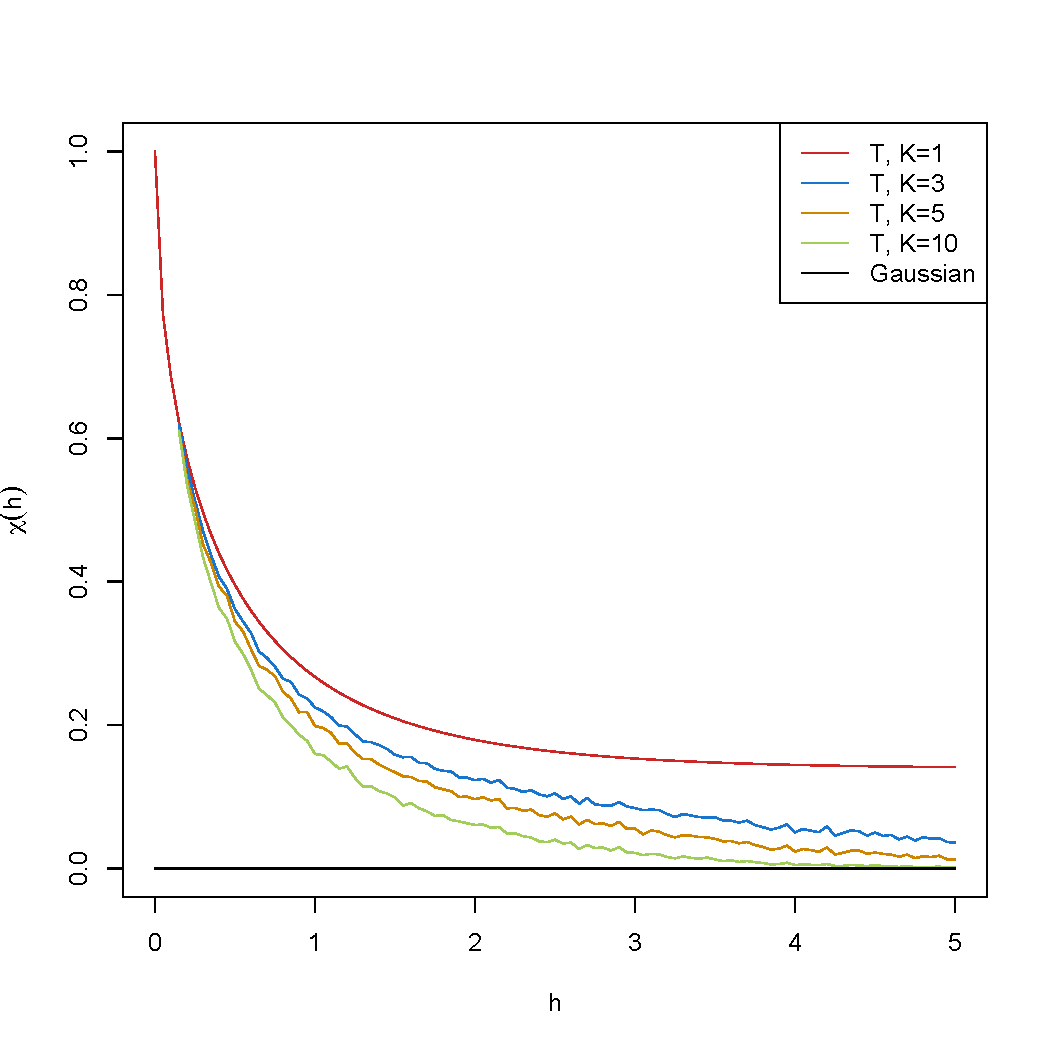
\includegraphics[width=0.5\linewidth]{plots/chi-h.pdf}
  \caption{$\chi(h)$ for $K = 1, 3, 5$, and $10$ knots as a function of distance.}
  \label{fig:chi}
\end{figure}

\subsection{Extension to space-time data} \label{s:temporal}
When using daily measurements, the assumption of temporal independence is often inappropriate.
There are several places where temporal dependence could be incorporated in the model, including the residual $v_t(\bs)$.
However, we choose to allow for temporal dependence in the $\bw$, $z$, and $\sigma$ terms because these terms dictate the tail behavior which is our primary focus.
In this section, we extend (\ref{eq:partition}) to the spatiotemporal setting.
Let
\begin{align} \label{eq:spatiotemp}
  Y_t(\bs) = \bX_t(\bs)^T \bbeta + \lambda \sigma_t(\bs) |z_t(\bs)| + \sigma_t(\bs) v_t(\bs),
\end{align}
where $t \in \{1, \ldots, T\}$ denotes the day of each observation.
Let \hbox{$\bw_{tk} = (w_{tk1}, w_{tk2})$} be a spatial knot on day $t$, and let $w_{t1}, \ldots, w_{tK}$ be a collection of spatial knots on day $t$.
As in section \ref{s:part}, these knots define a daily partition $P_{t1}, \ldots, P_{tK}$, and for $\bs \in P_{tk}$,
\begin{align}
  z_t(\bs) = z_{tk}\quad \text{and} \quad \sigma_{t}(\bs) = \sigma_{tk}.
\end{align}
We allow the partition structure to vary from day to day in order to account for sharp spikes in ozone that may not be present every day (e.g. a forest fire).

We use an AR(1) time series model for $w_{tk}$, $z_{tk}$, and $\sigma_{tk}$.
The time series model must be specified after a transformation to preserve the skew-$t$ process at each time point.
For each time-varying parameter, we transform to obtain a standard normal marginal distribution, place a Gaussian prior with autocorrelation on the transformed parameter, and then transform back to obtain the marginal distribution required to preserve the skew-$t$ process.
We first transform the spatial knots from $\calD$ to $\calR^2$ as follows.
Let
\begin{align}
  w^*_{tki} = \Phi^{-1}\left[ \frac{ w_{tki} - \min(\bs_i)}{ \max(\bs_i) - \min(\bs_i) } \right], \quad i = 1, 2
\end{align}
where $\Phi$ is a univariate standard normal density function, and $\bs_i = [s_{1i}, \ldots, s_{ni}]$.
Then the transformed knots $\bw^*_{tk} \in \calR^2$.
We use a copula on $\sigma^2_t(\bs)$ to ensure that the marginal distributions of $\sigma^2_t(\bs)$ are inverse gamma.
Let
\begin{align}
  \sigma^{2*}_t(\bs) =\Phi^{-1}\left\{ \text{IG}[\sigma^2_t(\bs)] \right\}
\end{align}
where IG is defined as before.
We also use a copula on $z_{t}(\bs)$ to ensure that the marginal distributions of $z_t(\bs)$ are half-normal.
Let
\begin{align}
  z^*_t(\bs) = \Phi^{-1}\left\{ \text{HN}[z_t(\bs)] \right\}
\end{align}
where HN is the distribution function of a half-normal random variable.
The AR(1) process for each tail parameter is $\bw^*_{1k} \sim N_w(0, 1)$, $z^*_{1k} \sim N(0, \sigma^2_{1k})$, $\sigma^{2*}_{1k} \sim N(0, 1)$, and for $t > 1$ the time series is modeled as
\begin{align}
  \bw^*_{tk} | \bw^*_{t-1, k} &\sim N_2\left[\phi_w \bw^*_{t-1, k}, (1 - \phi_w^2) \right] \\
  z^*_{tk} | z^*_{t-1, k} &\sim N \left[\phi_z z^*_{t-1, k}, \sigma^2_{tk} (1 - \phi_z^2)\right] \\
  \sigma^{2*}_{tk} | \sigma^{2*}_{t-1, k} &\sim N \left[\phi_\sigma \sigma^{2*}_{t-1, k}, (1 - \phi_\sigma^2) \right]
\end{align}
where $|\phi_w|$, $|\phi_z|$, $|\phi_\sigma| < 1$.
These are stationary time series models with marginal distributions \hbox{$\bw^*_{k} \sim N_2(0, 1)$}, \hbox{$z^*_{k} \sim N(0, \sigma^2_{k})$}, and \hbox{$\sigma^{2*}_{k} \sim N(0, 1)$}.
After transformation back to the original space, $\bw_{tk} \sim \text{Unif}(\calD)$, $z_{tk} \sim HN(0, \sigma^2_{tk})$ $\sigma^2_{tk} \sim \text{IG}(a, b)$.
For each day, the model is identical to the spatial-only model in (\ref{eq:partition}) by construction.

\section{Computation}\label{s:comp}
First, we impute values below the threshold conditional on observations above the threshold.
This is feasible for large datasets with our model because for a single day, conditional on the model parameters, we only need to draw from a truncated multivariate normal distribution.
Then, we update model parameters, $\Theta$, using Metropolis Hastings or Gibbs sampling when appropriate.
Finally, we make spatial predictions using conditional multivariate normal results and the fact that the distribution of $Y_t(\bs) \mid \Theta, z(\bs)$ is the usual multivariate normal distribution with a \Matern spatial covariance structure.

We can use Gibbs sampling to update $Y_t(\bs)$ for censored observations that are below the threshold $T$.
After conditioning on $\lambda$, $z_t(\bs)$ and non-censored observations, $Y_t(\bs)$ has truncated normal full conditionals.
So we sample $Y_t(\bs) \sim N_{(-\infty, T)}(\bX_t^T(\bs) \beta + \lambda | z_t(\bs)|, \bSigma)$.
After imputing the censored observations, we update the model parameters.
To update the model parameters, we use standard Gibbs updates for parameters when possible.
In the case Gibbs sampling is not possible, parameters are updated using a random-walk Metropolis Hastings algorithm.
See Appendices A.1 and A.2 for details regarding the MCMC.
The final step of the computation is to use Bayesian Kriging to generate a predictive distribution for $Y_t(\bs^*)$ at prediction location $\bs^*$.
This step is similar to the imputation for censored observations except that the full conditionals are no longer truncated at $T$.

\subsection{Hierarchical model}\label{s:hier}
Conditioned on $z_{tk}(\bs)$, $\sigma^2_{tk}(\bs)$, and $P_{tk}$, the marginal distributions are Gaussian and the joint distribution multivariate Gaussian.
However, we do not fix the partitions, they are treated as unknown and updated in the MCMC.
We model this with a Bayesian hierarchical model as follows.
Let $\bw_{t1}, \ldots, \bw_{tK}$ be a set of daily spatial knots in a spatial domain of interest, $\calD$, and $P_{tk}$ as defined in (\ref{eq:subregions}).
In practice, we fix $K$ at many different levels, and assess the impact of fit as described in \ref{s:modelselect}.
Then
\begin{align}
   Y_t(\bs) \mid z_{t}(\bs), \sigma_t^2(\bs), P_{tk}, \Theta &= \bX_t(\bs)^T \beta + \lambda |z_t(\bs)| + \sigma_t(\bs) v_t(\bs) \label{eq:hier}\\
   z_t(\bs) &= z_{tk} \text{ if } \bs \in P_{tk}\nonumber\\
   \sigma^2_{t}(\bs) &= \sigma^2_{tk} \text{ if } \bs \in P_{tk}\nonumber\\
   \lambda &= \lambda_1 \lambda_2\nonumber\\
   \lambda_1 &= \left\{ \begin{array}{ll}
      +1 \quad & \text{w.p. } 0.5\\
      -1 \quad & \text{w.p. } 0.5
   \end{array}\right.\nonumber\\
   \lambda^2_2 & \sim IG(a, b)\nonumber\\
   v_t(\bs) \mid \Theta &\sim \Matern(0, \Sigma)\nonumber\\
   z^*_{tk} \mid z^*_{t-1, k}, \sigma^2_{tk} &\sim N(\phi_z z^*_{t-1, k}, \sigma^2_{tk} (1 - \phi_z^2))\nonumber\\
   \sigma^{2*}_{tk} \mid \sigma^{2*}_{t-1, k} &\sim N(\phi_\sigma \sigma^{2*}_{t-1, k}, (1 - \phi_\sigma^2))\nonumber\\
   \bw^*_{tk} \mid \bw^*_{t-1, k} &\sim N_2(\phi_w \bw^*_{t-1, k}, (1 - \phi_w^2)) \nonumber
\end{align}
where $\Theta = \{\rho, \nu, \gamma\, \lambda, \beta\}$, and $\Sigma$ is a \Matern covariance matrix as described in Section \ref{s:skewt}.
We parameterize $\lambda = \lambda_1 \lambda_2$ to help with convergence in the MCMC.

\section{Simulation study}\label{s:simstudy}
In this section, we conduct a simulation study to investigate how the number of partitions and the level of thresholding impact the accuracy of predictions made by the model.

\subsection{Design}\label{s:simdesign}
For all simulation designs, we generate data from the model in Section \ref{s:part} using $n_s=144$ sites and $n_t=50$ independent days.
The sites are generated Uniform$([0, 10] \times [0, 10])$.
We generate data from 5 different simulation designs:
\begin{enumerate} \setlength{\itemsep}{-0.5em}
  \item Gaussian marginal, $K=1$ knot
  % \item Symmetric-$t$ marginal, $K=1$ knot
  % \item Symmetric-$t$ marginal, $K=5$ knots
  \item Skew-$t$ marginal, $K=1$ knots
  \item Skew-$t$ marginal, $K=5$ knots
  \item Max-stable
  \item Transformation below $T = q(0.80)$
\end{enumerate}
In the first three designs, the $v_t(\bs)$ terms are generated using a \Matern covariance with smoothness parameter $\nu = 0.5$ and spatial range $\rho = 1$.
For the covariance matrices in designs 1 -- 3, the proportion of the variance accounted for by the spatial variation is $\gamma = 0.9$ while the proportion of the variance accounted for by the nugget effect is $0.1$.
In the first design, $\sigma^2 = 2$ is used for all days which results in a Gaussian distribution.
For designs 2 and 3, $\sigma^2_{tk} \iid \text{IG}(3, 8)$ to give a $t$ distribution with 6 degrees of freedom.
For designs 1, we set $\lambda = 0$.
For designs 2 and 3, $\lambda = 3$ was used as to simulate moderate skewness, and the $z_t$ are generated as described in (\ref{eq:sitezsig}).
In the fourth design, we generate from a spatial max-stable distribution \citep{Reich2012}.
In this design, data have marginal distributions that follow a generalized extreme value distribution with parameters $\mu = 1, \sigma=1, \xi=0.2$.
In this model, a random effect is used to induce spatial dependence using 144 spatial knots on a regular lattice in the square $[1, 9] \times [1, 9]$.
For this setting, we set $\gamma = 0.5$.
In the final design, we generate $\tilde{y}$ using the setting from design two, and then consider the data
\begin{align}
  y = \left\{ \begin{array}{lc}
    \tilde{y}, \quad & \tilde{y} > T \\[0.5em]
    T \exp\{\tilde{y} - T\}, \quad & \tilde{y} \le T
  \end{array}\right.
\end{align}
where $T = q(0.80)$ is the 80th sample quantile of the data.
In all five designs, the mean $\bX^T \bbeta = 10$ is assumed to be constant across space.

$M = 50$ data sets are generated for each design.
For each data set we fit the data using five models
\begin{enumerate} \setlength{\itemsep}{-0.5em}
  \item Gaussian marginal, $K=1$ knots
  \item Skew-$t$ marginal, $K=1$ knots, $T=-\infty$
  \item Symmetric-$t$ marginal, $K=1$ knots, $T=q(0.80)$
  \item Skew-$t$ marginal, $K=5$ knots, $T=-\infty$
  \item Symmetric-$t$ marginal, $K=5$ knots, $T=q(0.80)$
  \item A max-stable model based on \citet{Reich2012} thresholded at $T = q(0.80)$
\end{enumerate}
where $q(0.80)$ is the 80th sample quantile of the data.
The design matrix $\bX$ includes an intercept with a first-order spatial trend with priors of $\beta_\text{int}$, $\beta_\text{lat}$, $\beta_\text{long},  \iid \text{N}(0, 10)$.
The spatial covariance parameters have priors $\log(\nu) \sim \text{N}(-1.2, 1)$, $\gamma \sim \text{Unif}(0, 1)$, $\rho \sim \text{Unif}(15)$.
The skewness parameter has prior $\lambda_2 \sim \text{IG}(0.1, 0.1)$.
The residual variance terms have priors $\sigma^2_t(\bs) \sim \text{IG}(0.1, 0.1)$.
The knots have priors $\bw \sim \text{Unif}(\calD)$.
We tried also fitting the skew-$t$ marginals for the thresholded models, but it is very challenging for the MCMC to properly identify the skewness parameter with only one tail worth of data.
Each chain of the MCMC ran for 20000 iterations with a burn-in period of 10000 iterations.
Parameters appear to converge properly; however, in the models with multiple partitions (i.e.models 4 and 5) it is hard to assess the convergence of $\bw$, $z(\bs)$, and $\sigma^2(\bs)$ because of partition label switching throughout the MCMC.

\subsection{Cross validation}\label{s:modelselect}
Models were compared using cross validation with 100 sites used as training sites and 44 sites witheld for testing.
The model was fit using the training set, and predictions were generated at the testing site locations.
Because one of the primary goals of this model is to predict exceedances over a fixed threshold, we use Brier scores to select the model that best fits the data \citep{Gneiting2007}.
The Brier score for predicting exceedance of a threshold $c$ is given by $[e(c) - P(c)]^2$ where $e(c) = I[y>c]$ is an indicator function indicating that a test set value, $y$, has exceeded the threshold, $c$, and $P(c)$ is the predicted probability of exceeding $c$.
We average the Brier scores over all test sites and days.
For the Brier score, a lower score indicates a better fit.

\subsection{Results}\label{s:simresults}
We compared the Brier scores for exceeding 4 different thresholds for each dataset.
The thresholds used for the Brier scores are extreme quantiles from the simulated data for $q(0.90)$, $q(0.95)$, $q(0.98)$, and $q(0.99)$.
Figure \ref{fig:simbrierscores} gives the Brier score relative to the Brier score for the Gaussian method calculated as
\begin{align}
  \text{BS}_{\text{rel}} = \frac{\text{BS}_{\text{method}}}{\text{BS}_{\text{Gaussian}}}.
\end{align}
We analyzed the results for the simulation study using a Friedman test at $\alpha = 0.05$.
If the Friedman test came back with a significant results, we conducted a Wilcoxon-Nemenyi-McDonald-Thompson test to see which methods had different results.
The full results for the Wilcoxon-Nemenyi-McDonald-Thompson tests are given in Appendix \ref{a:pdiffs}.

Figure \ref{fig:simbrierscores} shows that when the data come from a Gaussian process, our methods perform comparably to the Gaussian method.
For data settings with skew-$t$ marginals (settings 2 -- 3), we find significant improvement over the Gaussian method.
Furthermore in these data settings, we find the best performance occurs when the number of knots used in the method matches the number of knots used for data generation.
The non-thresholded methods tend to outperform the thresholded methods, but this is not surprising given that the data are generated directly from the model used in the method.
For the max-stable data, we see that for low-extreme quantiles, the Gaussian method performs better, for more extreme quantiles, the single-partition method, both thresholded and non-thresholded, perform significantly better than the Gaussian.
Finally, for setting 5, although the thresholded version of the single-partition model tends to perform the best across all of the extreme quantiles, the difference between the thresholded and non-thresholded methods is no longer significant in the more extreme quantiles.

\begin{figure}
  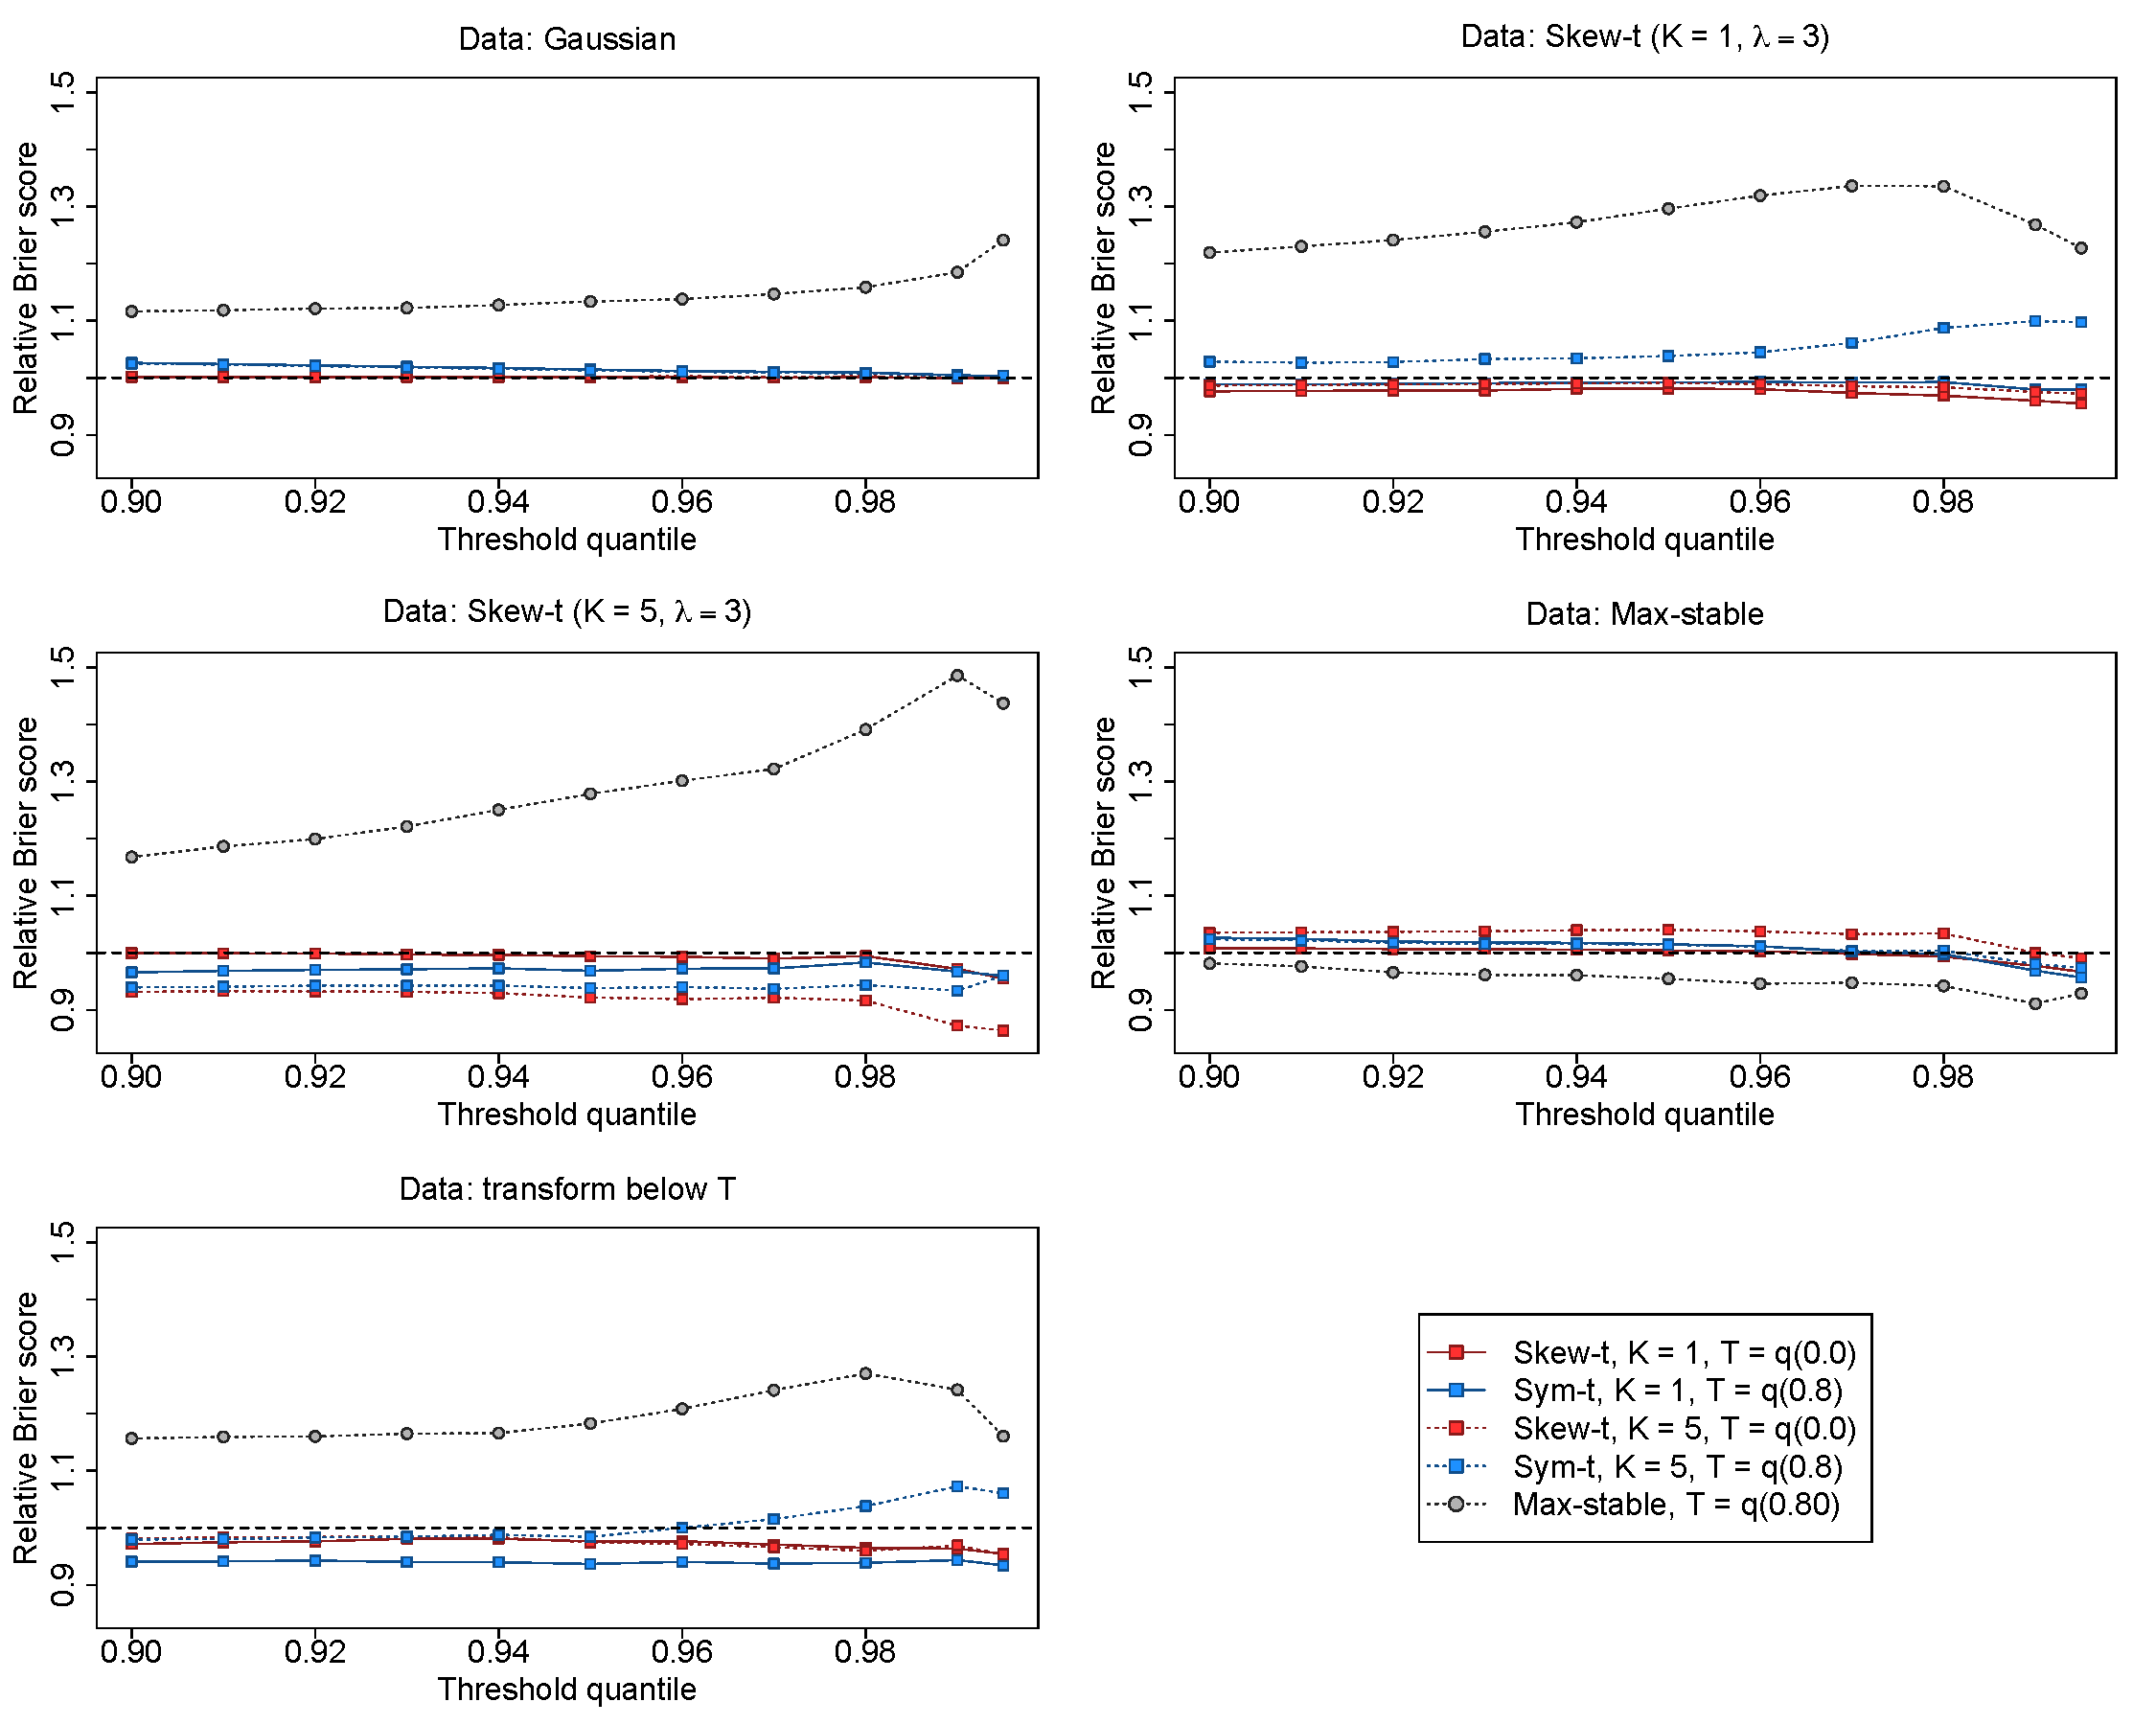
\includegraphics[width=\linewidth]{plots/bsplots-mean.pdf}
  \caption{Brier scores relative to the Gaussian method for simulation study results. A ratio lower than 1 indicates that the method outperforms the Gaussian method.}
  \label{fig:simbrierscores}
\end{figure}

\section{Data analysis}\label{s:analysis}
To illustrate this method, we consider the daily maximum 8-hour ozone measurements for July 1 - 31, 2005 at 1089 Air Quality System (AQS) monitoring sites in the United States as the response (see Figure \ref{fig:ozone}).
For each site, we also have covariate information containing the estimated ozone from the Community Multi-scale Air Quality (CMAQ) modeling system.
Initially, we fit a linear regression assuming a mean function of
\begin{align}
  \bX^T_t(\bs) \bbeta = \beta_0 + \beta_1 \cdot \text{CMAQ}_t(\bs). \label{eq:datamean}
\end{align}
The data from July 10 are shown in Figure \ref{fig:ozone} along with a Q-Q plot of the residuals compared to a skew-$t$ distribution with 10 d.f. and $\alpha = 1$.
\begin{figure}
  \centering
  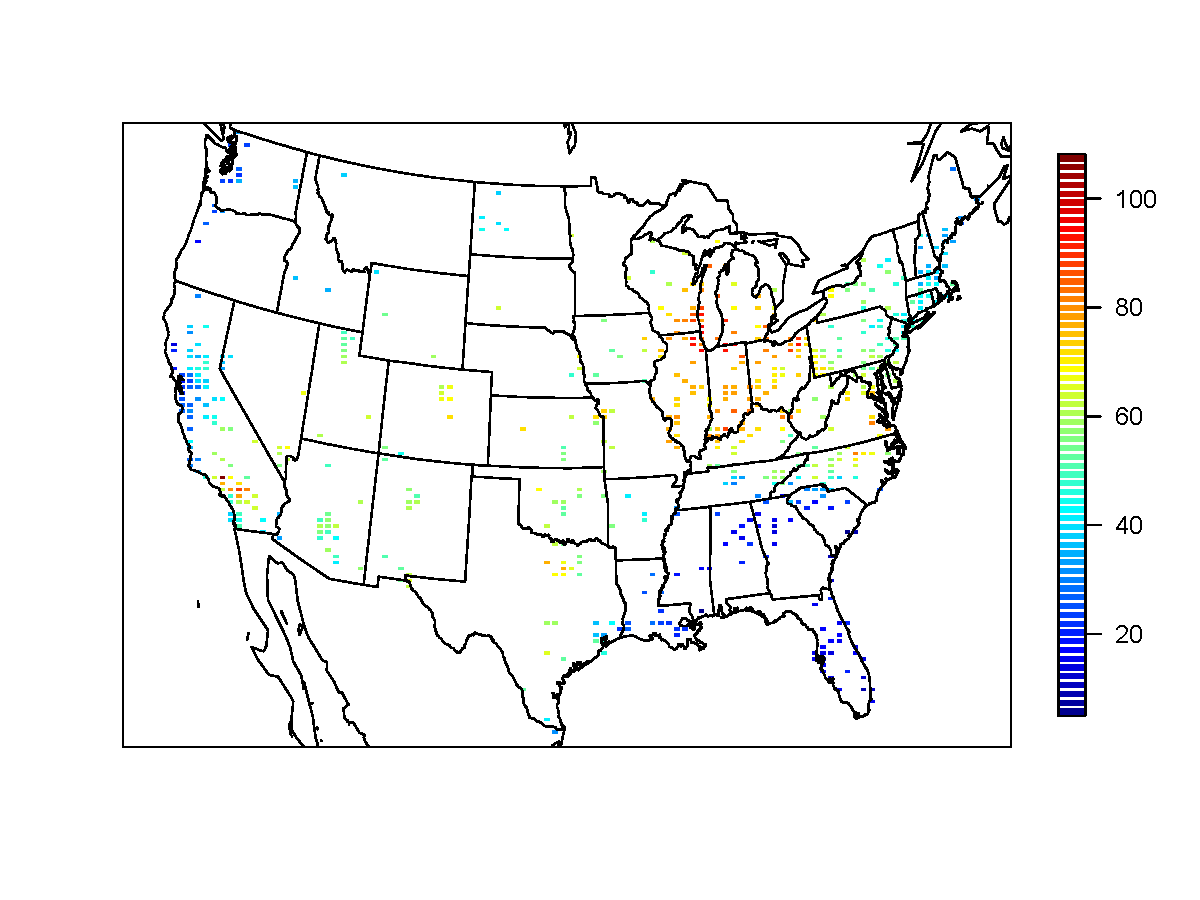
\includegraphics[width=0.56\linewidth]{plots/ozone-10jul-us.pdf}
  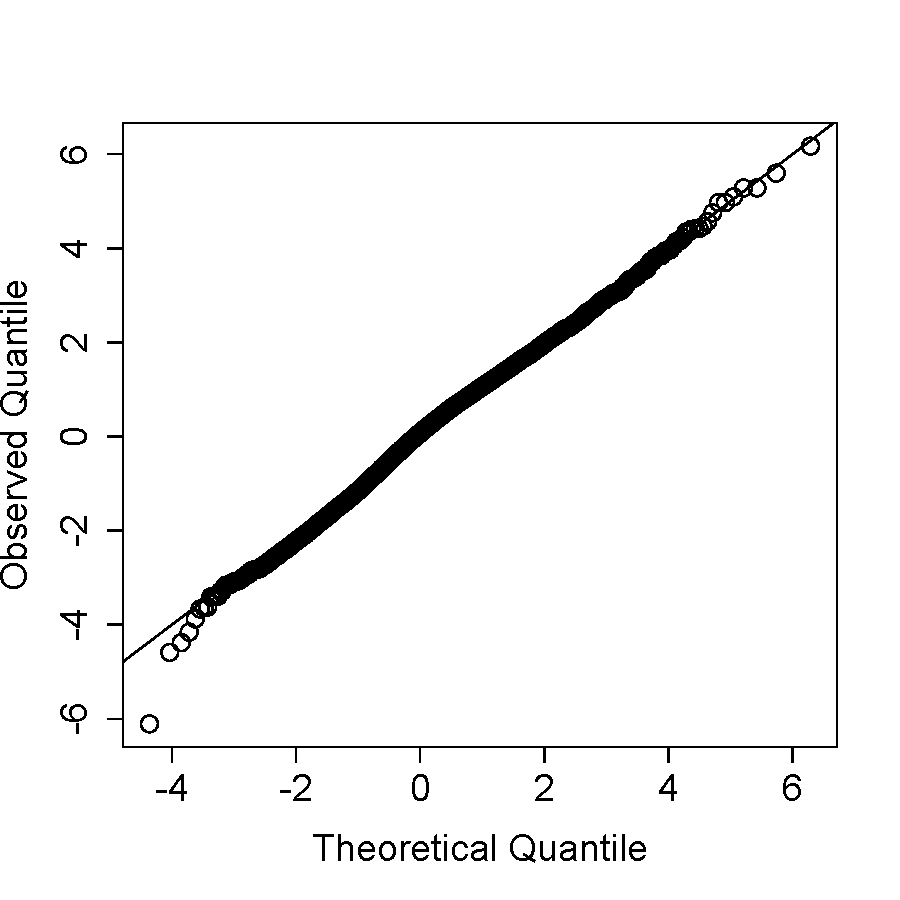
\includegraphics[width=0.41\linewidth]{plots/qq-res.pdf}
  \caption{Ozone values on 10 July 2005 (left) Q-Q plot of the residuals (right)}
  \label{fig:ozone}
\end{figure}
Exploratory data analysis indicates that there is dependence in the high quantile levels of the residuals beyond what we expect in the case of independence.

% We explore spatial and temporal extremal dependence by considering $\chi_c = \Pr[Y(\bs) > c | Y(\bt) > c]$.
% To examine spatial dependence in high quantiles, we consider observations at all pairs of sites $\bs$ and $\bt$ that are distance $h$ apart where $h$ is separated into bins of size 0.25 km.
% Then conditioned on $Y(\bt) > c$, we take the sample proportion of $Y(\bs) > c$.
% Finally, $\widehat{\chi}_c(h)$ is averaged over all days at each of the three threshold quantiles.
% To examine temporal dependence in high quantiles, we consider observations at a single site that are taken lag-$t$ days apart.
% Then conditioned on $Y_n(\bs) > c$, we take the sample proportion of $Y_{n + t}(\bs) > c$.
% Finally, $\widehat{\chi}(t)$ is averaged over all sites at each of the three threshold quantiles.
% The $\widehat{\chi}_c(h)$ and $\widehat{\chi}_c(t)$ plots in Figure \ref{fig:chi-st} show the estimated spatial and temporal dependence of the residuals for the ozone data at three quantile levels $q(0.90), q(0.95)$, and $q(0.99)$.

% \begin{figure}
%   \centering
%   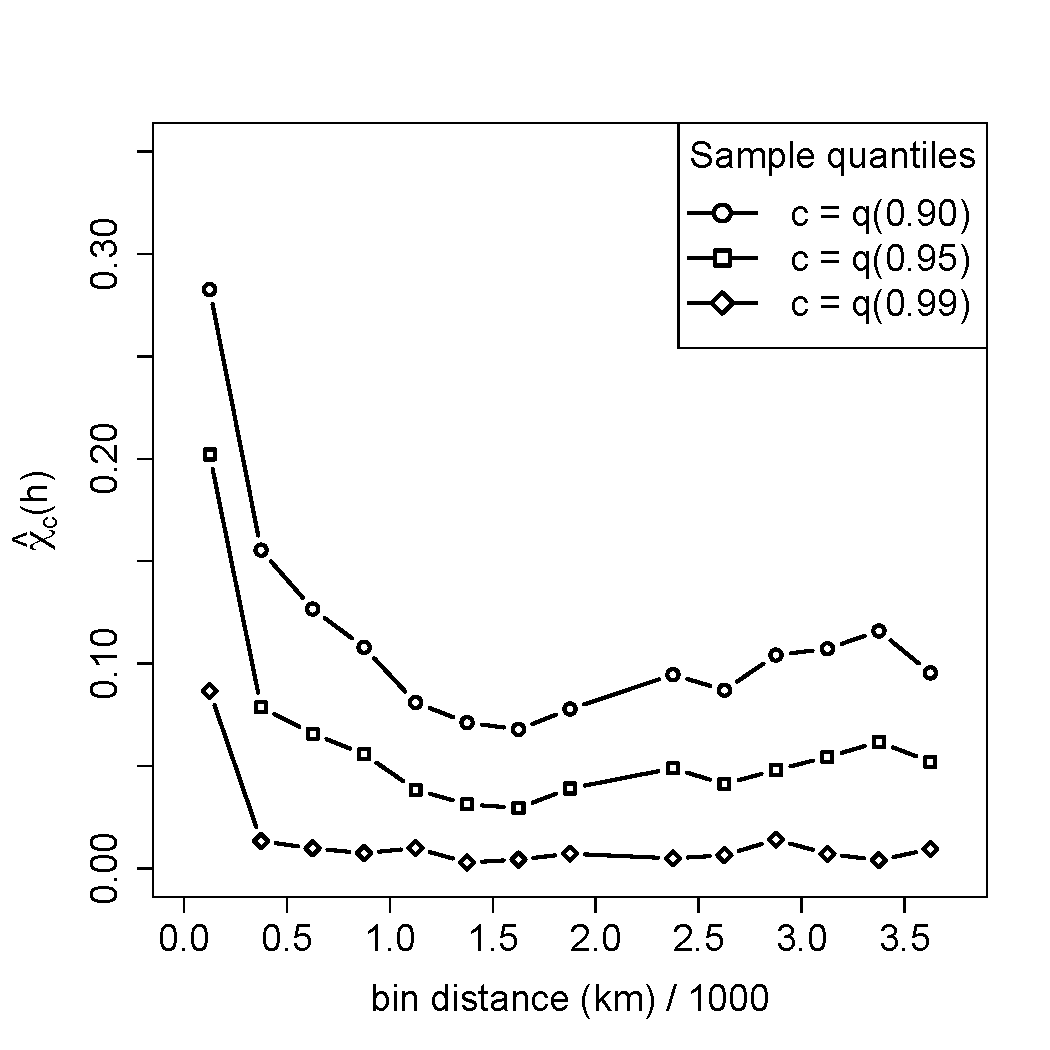
\includegraphics[width=0.49\linewidth]{plots/chi-h-ozone.pdf}
%   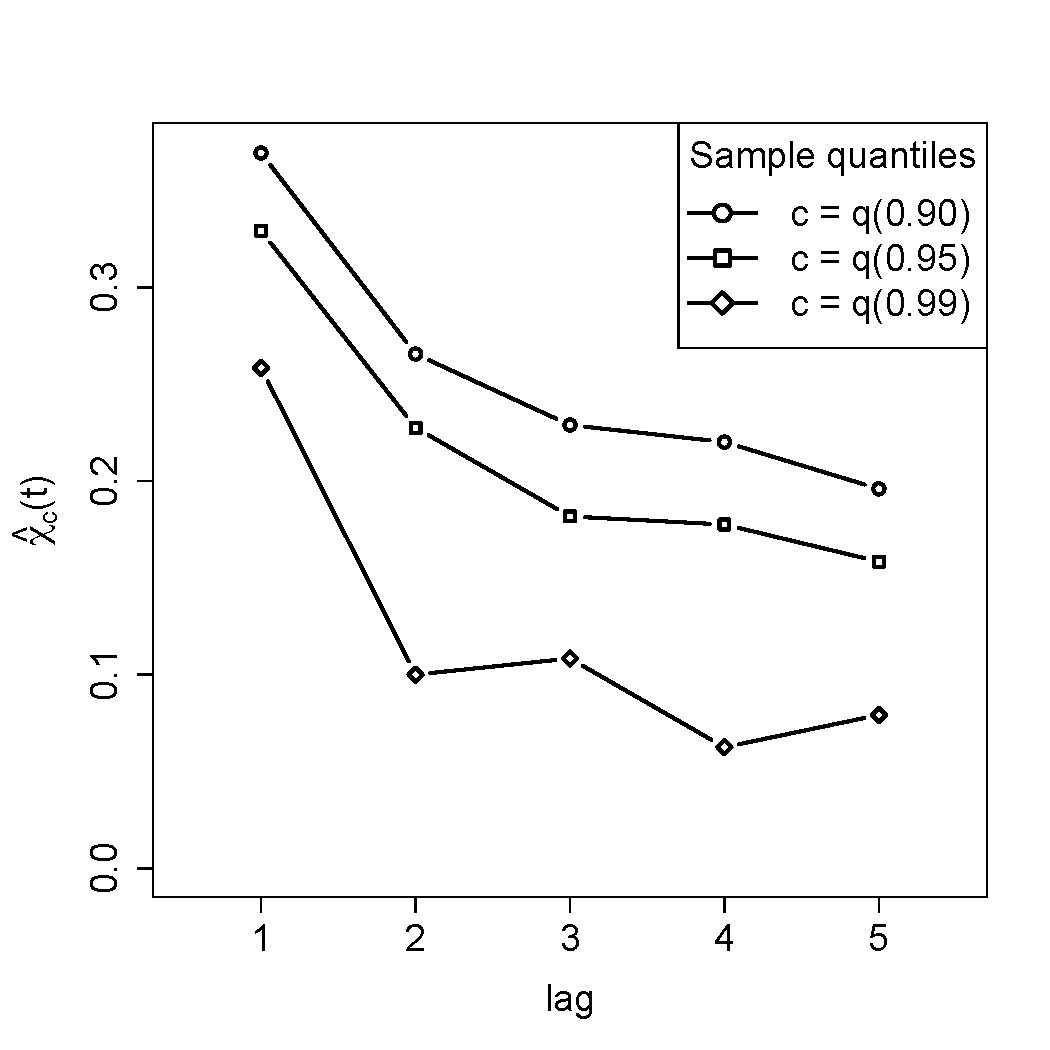
\includegraphics[width=0.49\linewidth]{plots/chi-t-ozone.pdf}
%   \caption{$\widehat{\chi}_c(h)$ plot for the residuals (left). $\widehat{\chi}_c(t)$ plot for the residuals (right).}
%   \label{fig:chi-st}
% \end{figure}

\subsection{Model comparisons}
We fit the model using Gaussian and skew-$t$ marginal distributions with $K=1, 5, 6, 7, 8, 9, 10, 15$ partitions.
We choose to censor $Y(\bs)$ at $T =$ 0, 50 (0.42 sample quantile), and 75 (0.92 sample quantile) ppb in order to compare results from no, moderate, and high censoring.
The upper threshold of 75 ppb was used because the current air quality standard is based on exceedance of 75 ppb.
As with the simuliation study, for models with a threshold of $T = 75$, we use a symmetric-$t$ marginal distribution.
We also compare models with no time series to models that include the time series.
Finally, as a comparison to max-stable methods, we fit the model using the hierarchical max-stable model of \citet{Reich2012} with the data thresholded at $T = 75$.
All methods assume the mean function given in (\ref{eq:datamean}).
To ensure that the max-stable method runs in a reasonable amount of time, we take a stratified sample of the sites to get 800 sites and consider this our new dataset.
We conduct two-fold cross validation using 400 training sites and 400 validation sites as described in Section \ref{s:modelselect}

Each chain of the MCMC ran for 30000 iterations with a burn-in period of 25000 iterations.
Parameters appear to converge properly; however, as before, for models with multiple partitions it is hard to assess the convergence of $\bw$, $z(\bs)$, and $\sigma^2(\bs)$ because of partition label switching throughout the MCMC.
For each model, Brier scores were averaged over all sites and days to obtain a single Brier score for each dataset.
At a particular threshold or quantile level, the model that fits the best is the one with the lowest score.
We then compute the relative (to Gaussian) Brier scores (see Section \ref{s:simresults}) to compare each model.

\subsection{Results}\label{s:results}
The results suggest that the skew-$t$, thresholded, partitioned, and time series models all give an improvement in predictions over the Gaussian model, whereas the max-stable method results in relative Brier scores between 1.07 and 1.15 indicating poorer performance than the Gaussian model.
The plots in Figure \ref{fig:bs-ozone} show the relative Brier scores for time-series and non-time-series models, using $K = $ 1, 7, and 15 knots at thresholds $T = $ 0, 50, and 75 ppb.
Most of the models perform similarly across all the Brier scores; however, for single-partition models without thresholding, performance tends to diminish in the extreme quantiles.
The results also suggest that thresholding improves performance for estimates in the extreme quantiles.
Both plots have similar features suggesting that most settings do reasonably well.
In particular, for all extreme quantiles, selecting a moderate number of knots (e.g. $K = 5, \ldots, 10$) tends to give the best results.
Table \ref{tbl:ozoneresults} shows the best two models for selected extreme quantiles.

We illustrate the predictive capability of our model in Figure \ref{fig:ozoneq99} by plotting the 99th quantile of the posterior predictive density for July in South Carolina and Georgia.
We fit the model using four methods, two reference and two that performed better.
These four methods are
\begin{enumerate}\setlength{\itemsep}{-0.5em}
  \item Gaussian (reference)
  \item Skew-$t$, $K =$ 1 knot, $T = $ 0, no time series (reference)
  \item Skew-$t$, $K =$ 5 knots, $T = $ 50, no time series (comparison)
  \item Symmetric-$t$, $K =$ 10 knots, $T = $ 75, time series (comparison).
\end{enumerate}
In the bottom two plots, we plot the differences between method 4 and methods 1 and 2.
The most noticeable differences between the reference methods and the comparison methods is that the comparison methods tend to give higher estimates of the 99th quantile along the I-85 corridor between Charlotte and Atlanta.

\begin{figure}
  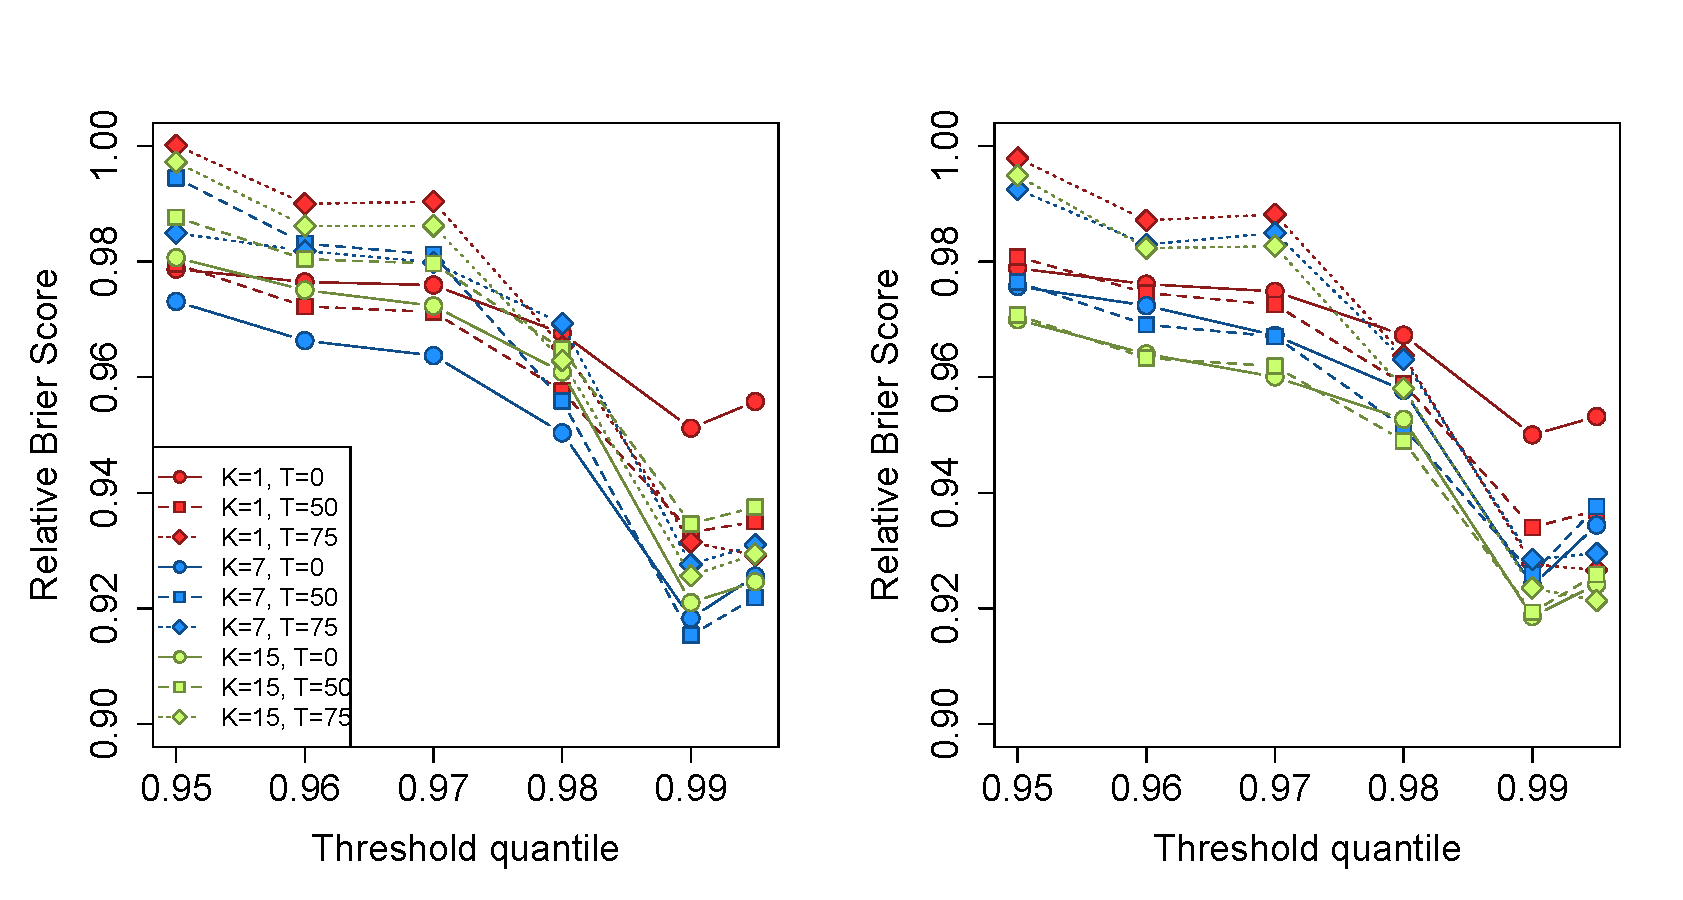
\includegraphics[width=\linewidth]{plots/bs-ozone.pdf}
  \caption{Relative Brier scores for time-series models (left) and non-time-series models (right). Relative brier score for the max-stable model is between 1.07 and 1.15}
  \label{fig:bs-ozone}
\end{figure}
\begin{table}
  \small
  \caption{Top two performing models for ozone analysis at extreme quantiles with Relative Brier score}
  \label{tbl:ozoneresults}
  \centering
  \begin{tabular}{|l|l l l c|l l l c|}
    \cline{2-9}
    \multicolumn{1}{c|}{}  & \multicolumn{4}{c|}{1st} & \multicolumn{4}{c|}{2nd} \\
    \hline
    $q(0.90)$  & No time series & $K=7$  & $T=0$  & BS: 0.980 &
                 No time series & $K=9$  & $T=0$  & BS: 0.980 \\
    $q(0.95)$  & No time series & $K=15$ & $T=50$ & BS: 0.970 &
                 No time series & $K=9$  & $T=50$ & BS: 0.970\\
    $q(0.98)$  & No time series & $K=5$  & $T=50$ & BS: 0.945 &
                 No time series & $K=10$ & $T=50$ & BS: 0.946\\
    $q(0.99)$  & Time series    & $K=10$ & $T=75$ & BS: 0.912 &
                 Time series    & $K=6$  & $T=75$ & BS: 0.913\\
    $q(0.995)$ & Time series    & $K=6$  & $T=75$ & BS: 0.917 &
                 Time series    & $K=10$ & $T=75$ & BS: 0.918\\
    \hline
  \end{tabular}
\end{table}

\begin{figure}
  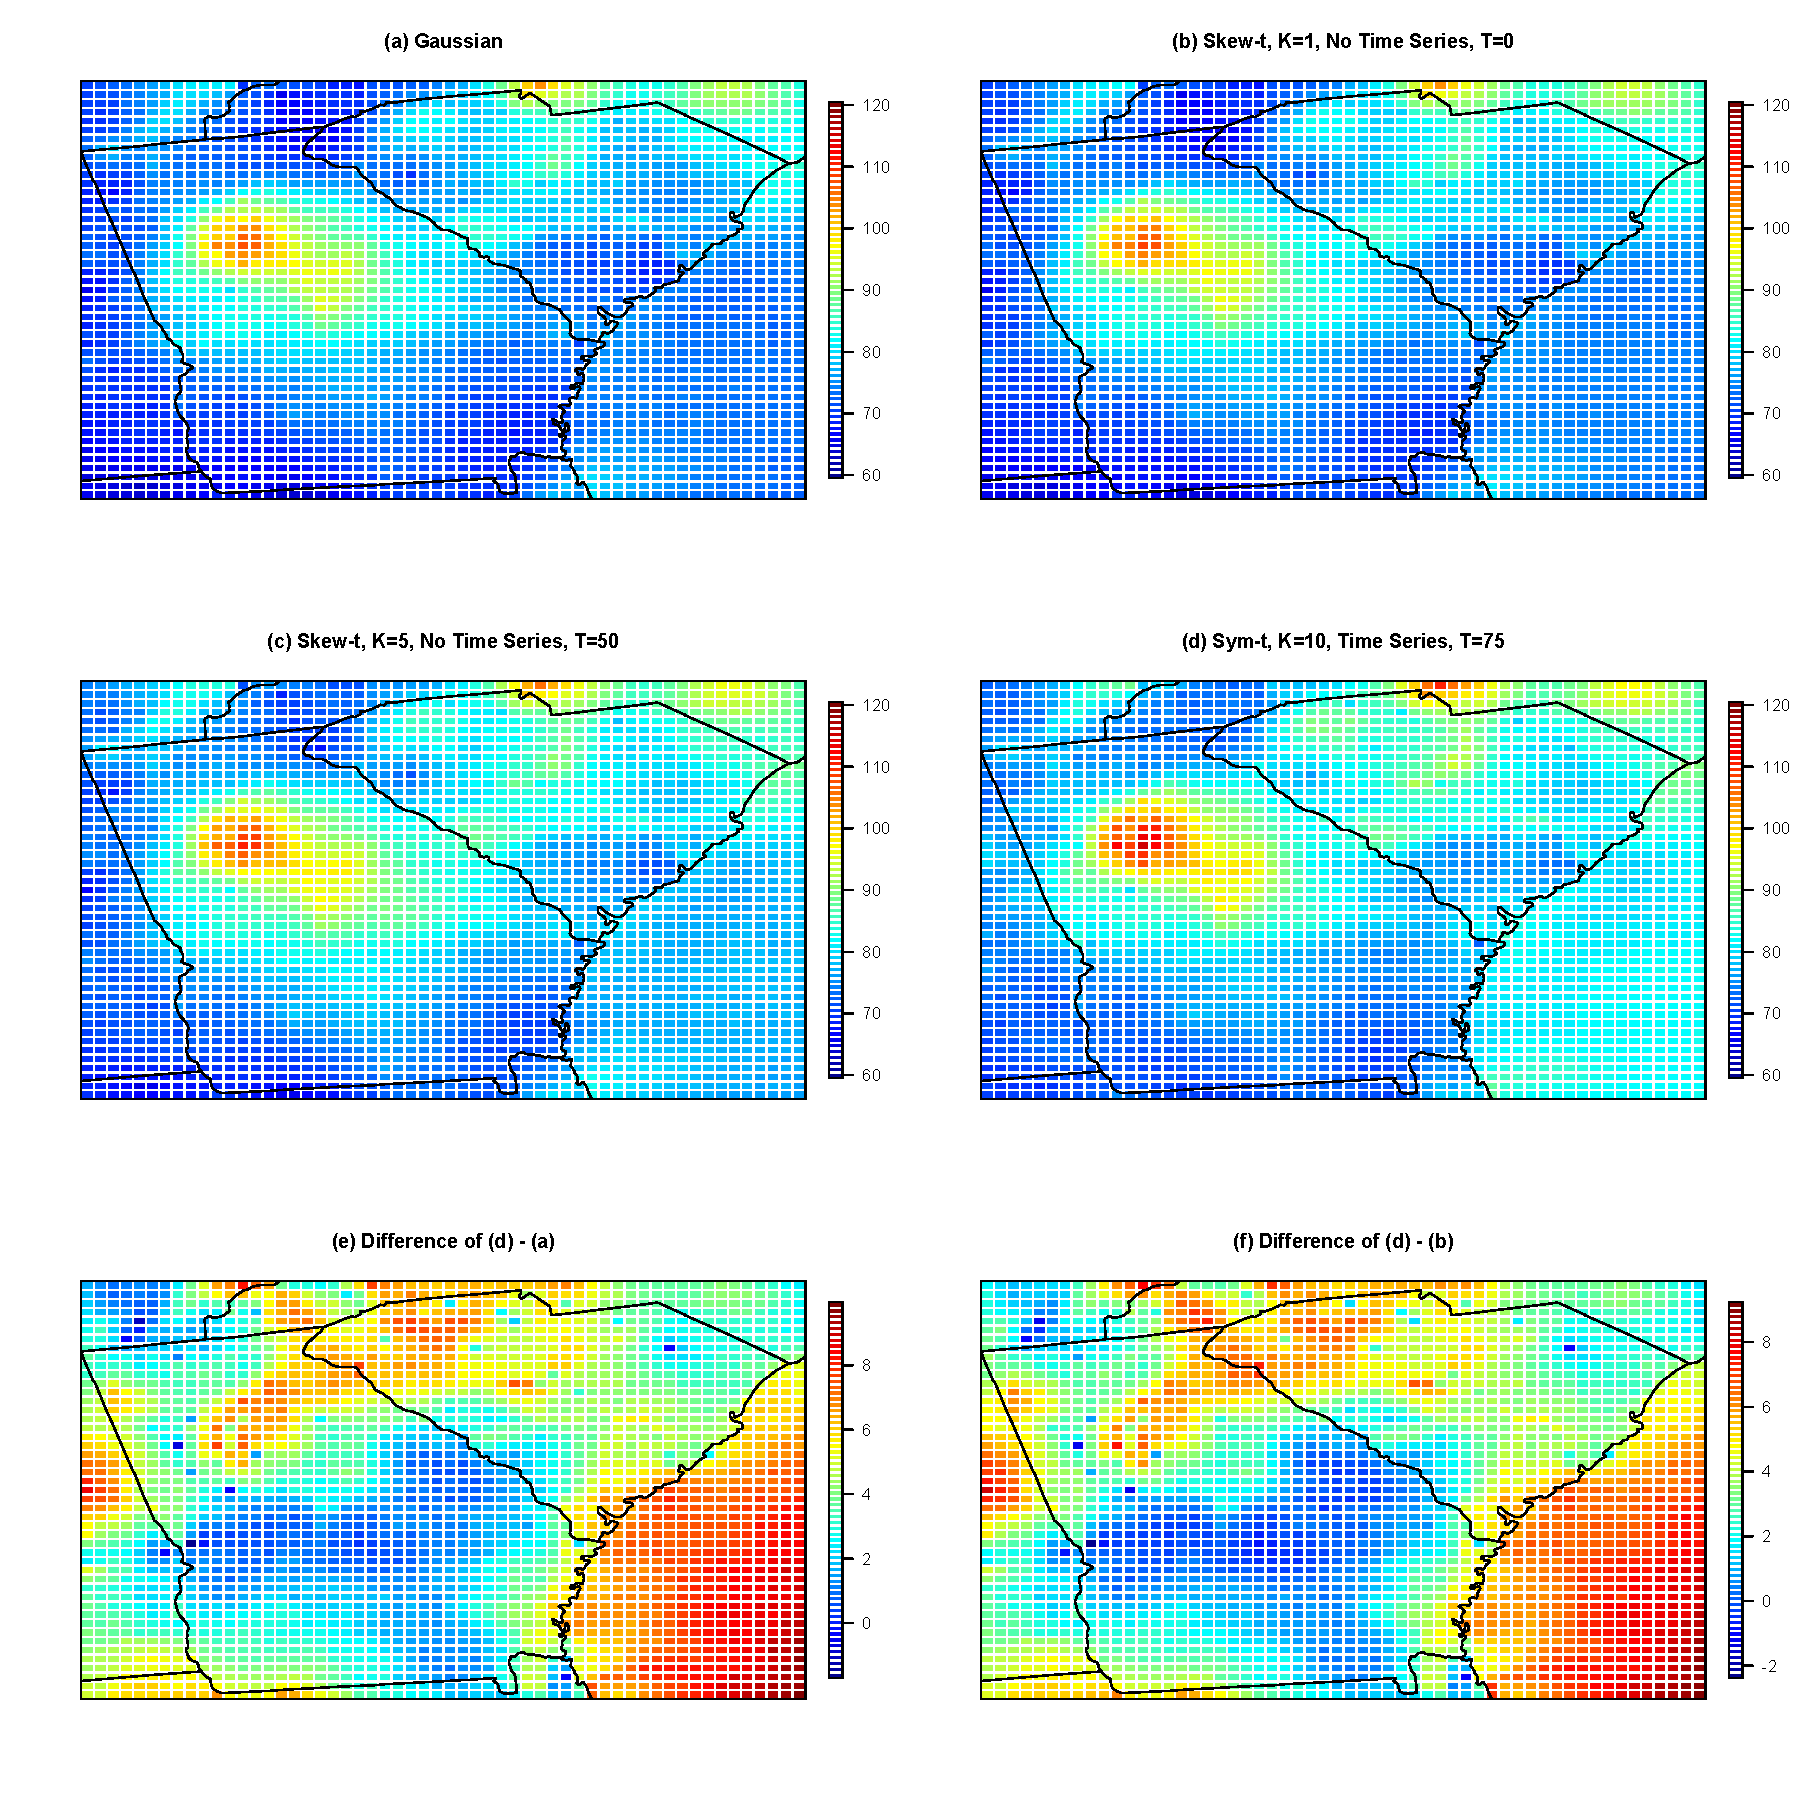
\includegraphics[width=\linewidth]{plots/q99-ozone.pdf}
  \caption{(a) -- (d) give give the posterior predictive $\widehat{q}(0.99)$ for the month of July under four different models, (e) gives the difference between $\widehat{q}(0.99)$ in plots (d) and (a), (f) gives the difference between $\widehat{q}(0.99)$ in plots (d) and (b).}
  \label{fig:ozoneq99}
\end{figure}

\section{Discussion}\label{s:con}
In this paper we propose a new threshold exceedance approach for spatiotemporal modeling based on the skew-$t$ process.
The proposed model gives flexible tail behavior, demonstrates asymptotic dependence for observations at sites that are near to one another, and has computation on the order of Gaussian models for large space-time datasets.
In the simulation study, we demonstrate that this model shows statistically significant improvements over a na\"{i}ve Gaussian approach.
In both the simulation study, and the application to ozone data, we find that incorporating a partition in the model improves extreme prediction.
Furthermore the results from the data analysis suggest that thresholding can improve performance when predicting in the extreme tails of the data.

This model presents new avenues for future research.
One possibility is the implementation of a different partition structure.
We choose to define the random effects for a site by using an indicator function based on closeness to a knot.
However, this indicator function could be replaced by kernel function that would allow for multiple knots to impact each site, with the weight of each knot to be determined by some characteristic such as distance.
Another area that should be explored is the temporal dependence in the model.
Instead of implementing a time series on the random effects, a three-dimensional covariance structure on the residuals could be implemented to address temporal dependence.
Finally, we acknowledge that by specifying the number of knots, we may be underestimating the uncertainty in the model.
This could be incoporated by treating the number of knots as a model parameter instead of fixing it to be a specific value.

\section*{Acknowledgments}

\appendix
\section{Appendices}
\subsection{MCMC details} \label{a:mcmc}
The MCMC sampling for the model \ref{s:hier} is done using {\tt R} (http://www.r-project.org). Whenever possible, we select conjugate priors (see Appendix \ref{a:posterior}); however, for some of the parameters, no conjugate prior distributions exist.
When no conjugate prior distribution exists, we use a random walk Metropolis Hastings update step.
In each Metropolis Hastings update, we tune the algorithm to give acceptance rates near 0.40.

\subsubsection*{Spatial knot locations}
For each day, we update the spatial knot locations, $\bw_1, \ldots, \bw_K$, using a Metropolis Hastings block update.
Because the spatial domain is bounded, we generate candidate knots using the transformed knots $\bw^*_1, \ldots, \bw^*_K$ (see section \ref{s:temporal}) and a random walk bivariate Gaussian candidate distribution
\begin{align*}
	{\bw^*_k}^{(c)} \sim \text{N}({\bw^*_k}^{(r - 1)}, s^2 I_2)
\end{align*}
where ${\bw^*_k}^{(r - 1)}$ is the location for the transformed knot at MCMC iteration $r - 1$, $s$ is a tuning parameter, and $I_2$ is an identity matrix.
After candidates have been generated for all $K$ knots, the acceptance ratio is
\begin{align*}
  R = \left\{ \frac{ l[ Y_t(\bs | \bw_1^{(c)}, \ldots, \bw_K^{(c)}, \ldots)] }{l[ Y_t(\bs | \bw_1^{(r - 1)}, \ldots, \bw_K^{(r - 1)}, \ldots)]} \right\} \times \left\{ \frac{ \prod_{k = 1}^{K}\phi(\bw_k^{(c)})}{ \prod_{k = 1}^{K}\phi(\bw_k^{(r - 1)})} \right\} \times \left\{ \frac{ \prod_{k = 1}^{K} p({\bw^*_k}^{(c)})}{ \prod_{k = 1}^{K} p({\bw^*_k}^{(r - 1)})}\right\}
\end{align*}
where $l$ is the likelihood given in (\ref{eq:hier}), and $p(\cdot)$ is the prior either taken from the time series given in (\ref{s:temporal}) or assumed to be uniform over $\calD$.
The candidate knots are accepted with probability $\min\{R, 1\}$.

\subsubsection*{Spatial random effects}
If there is no temporal dependence amongst the observations, we use a Gibbs update for $z_{tk}$, and the posterior distribution is given in \ref{a:posterior}.
If there is temporal dependence amongst the observations, then we update $z_{tk}$ using a Metropolis Hastings update.
Because this model uses $|z_{tk}|$, we generate candidate random effects using the $z^*_{tk}$ (see Section \ref{s:temporal}) and a random walk Gaussian candidate distribution
\begin{align*}
  {z^*_{tk}}^{(c)} \sim \text{N}({z^*_{tk}}^{(r - 1)}, s^2)
\end{align*}
where ${z^*_{tk}}^{(r-1)}$ is the value at MCMC iteration $r - 1$, and $s$ is a tuning parameter.
The acceptance ratio is
\begin{align*}
  R = \left\{ \frac{ l[Y_t(\bs) | z_{tk}^{(c)}, \ldots] }{ l[Y_t(\bs) | z_{tk}^{(r - 1)}]} \right\} \times \left\{ \frac{ p[ z_{tk}^{(c)} ] }{ p[ z_{tk}^{(r - 1)}]}\right\}
\end{align*}
where $p[\cdot]$ is the prior taken from the time series given in Section \ref{s:temporal}.
The candidate is accepted with probability $\min\{R, 1\}$.

\subsubsection*{Variance terms}
When there is more than one site in a partition, then we update $\sigma^2_{tk}$ using a Metropolis Hastings update.
First, we generate a candidate for $\sigma^2_{tk}$ using an IG$(a^*/s, b^*/s)$ candidate distribution in an independence Metropolis Hastings update where $a^* = (n_{tk} + 1) / 2 + a$, $b^* = [Y_{tk}^T \Sigma^{-1}_{tk} Y_{tk} + z_{tk}^2] / 2 + b$, $n_{tk}$ is the number of sites in partition $k$ on day $t$, and $Y_{tk}$ and $\Sigma^{-1}_{tk}$ are the observations and precision matrix for partition $k$ on day $t$.
The acceptance ratio is
\begin{align*}
  R = \left\{
    \frac{ l[Y_t(\bs) | {\sigma^2_{tk}}^{(c)}, \ldots] }
         { l[Y_t(\bs) | {\sigma^2_{tk}}^{(r - 1)}]}
    \right\} \times \left\{
    \frac{ l[z_{tk} | {\sigma^2_{tk}}^{(c)}, \ldots] }
         { l[z_{tk} | {\sigma^2_{tk}}^{(r - 1)}, \ldots] }
    \right\} \times \left\{
    \frac{ p[ {\sigma^2_{tk}}^{(c)} ] }
         { p[ {\sigma^2_{tk}}^{(r - 1)}] }
    \right\} \times \left\{
    \frac{ c[ {\sigma^2_{tk}}^{(r - 1)}] }
         { c[ {\sigma^2_{tk}}^{(c)}]}
    \right\}
\end{align*}
where $p[\cdot]$ is the prior either taken from the time series given in Section \ref{s:temporal} or assumed to be IG$(a, b)$, and $c[\cdot]$ is the candidate distribution.
The candidate is accepted with probability $\min\{R, 1\}$.

\subsubsection*{Spatial covariance parameters}
We update the three spatial covariance parameters, $\log(\rho)$, $\log(\nu)$, $\gamma$, using a Metropolis Hastings block update step.
First, we generate a candidate using a random walk Gaussian candidate distribution
\begin{align*}
	\log(\rho)^{(c)} \sim \text{N}(\log(\rho)^{(r - 1)}, s^2)
\end{align*}
where $\log(\rho)^{(r-1)}$ is the value at MCMC iteration $r - 1$, and $s$ is a tuning parameter.
Candidates are generated for $\log(\nu)$ and $\gamma$ in a similar fashion.
The acceptance ratio is
\begin{align*}
	R = \left\{ \frac{ \prod_{t = 1}^{T} l[Y_t(\bs) | \rho^{(c)}, \nu^{(c)}, \gamma^{(c)}, \ldots] }{\prod_{t = 1}^{T} l[Y_t(\bs) | \rho^{(r-1)}, \nu^{(r-1)}, \gamma^{(r-1)}, \ldots] } \right\} \times \left\{ \frac{ p[\rho^{(c)}] }{ p[\rho^{(r - 1)] } } \right\} \times \left\{ \frac{ p[\nu^{(c)}] }{ p[\nu^{(r - 1)}] } \right\} \times \left\{ \frac{ p[ \gamma^{(c)} ] }{ p[\gamma^{(r - 1)} ] } \right\}.
\end{align*}
All three candidates are accepted with probability $\min\{R, 1\}$.

\subsection{Posterior distributions} \label{a:posterior}



%\subsubsection*{Conditional posterior of $U | Y$}\label{s:condu}
% Let $Y_i | U \sim \mbox{N}(U, \sigma^2)$, $i = 1, \ldots, n$, let $\tau = 1 / \sigma^2$, and let $\pi(U) \propto \exp \left\{ -\frac{ u^2 \theta }{ 2 } \right\}$. 
% Then the conditional posterior of $U \mid \ldots$ is 
% \begin{align}
%   \pi (U \mid \ldots) & \propto \exp \left\{ -\frac{ u^2 \theta }{ 2 } \right\} \exp \left\{ - \sum_{i = 1 }^n\frac{ \tau (y_i - u)^2 }{ 2 } \right\} \nonumber \\
%     & \propto \exp \left\{ -\frac{ 1 }{ 2 } \left[ u^2 \theta + \sum_{i=1 }^n\tau (y_i^2 - 2y_iu + u^2) \right] \right\} \nonumber \\
%     & \propto \exp \left\{ - \frac{ 1 }{ 2 }\left( u - \frac{ \tau \sum_{i=1}^n y_i }{ \theta + n \tau } \right)^2 \left( \theta + n \tau \right) \right\} \nonumber\\
%     & \propto \mbox{HN}(\xi^*, \theta^*) \label{eq:condu}
% \end{align}
% where 
% \begin{align*}
%   \xi^* &= \frac{ \tau \sum_{i=1}^n y_i }{ \theta + n \tau }\\
%   \theta^* &= \theta + n \tauå
% \end{align*}

\subsubsection*{Conditional posterior of $z_{tl} \mid \ldots $}\label{s:mvcondu}
For simplicity, drop the subscript $t$ and define 
\begin{align*}
R(\bs) = \left\{ 
    \begin{array}{ll}
        Y(\bs) - X(\bs) \beta &s \in P_l\\[1em]
        Y(\bs) - X(\bs) \beta - \delta z(\bs) \qquad & s \notin P_l
    \end{array} 
\right.
\end{align*}
Let 
\begin{align*}
    R_1 &= \text{the vector of } R(\bs) \text{ for } s \in P_l \\
    R_2 &= \text{the vector of } R(\bs) \text{ for } s \notin P_l \\
    \Omega &= \Sigma^{-1}.
\end{align*}
Then
\begin{align*}
    \pi(z_l | \ldots) &\propto \exp \left\{ -\frac{ 1 }{ 2 \sigma^2 } \left[ \frac{ 1 }{ (1 - \delta^2)}
        \left( \begin{array}{c}
            R_1 - \delta z_l \bOne\\
            R_2
        \end{array} \right)^T
        \left( \begin{array}{cc}
            \Omega_{11} & \Omega_{12}\\
            \Omega_{21} & \Omega_{22}
        \end{array} \right)
        \left( \begin{array}{c}
            R_1 - \delta z_l \bOne\\
            R_2
        \end{array} \right)
        +  z_l^2 \right]
    \right\} I(z_l > 0) \\
        &\propto \exp \left\{ -\frac{ 1 }{ 2 \sigma^2 } \left[ \Lambda_z z_l^2 - 2 \mu_z z_l \right] \right\} I(z_l > 0)
\end{align*}
where
\begin{align*}
    \mu_z &= \frac{ \delta}{(1 - \delta^2)} ( R_1^T \Omega_{11} + R_2^T \Omega_{21} )\bOne\\
    \Lambda_z &= \frac{\delta^2 \bOne^T \Omega_{11} \bOne }{ (1 - \delta^2) } + 1.
\end{align*}
Then $Z_l | \ldots \sim N_{(0, \infty)} (\Lambda_z^{-1} \mu_z, \sigma^2 \Lambda_z^{-1})$
\subsection*{Conditional posterior of $\beta \mid \ldots$}\label{s:betapost}
Let $\beta \sim \mbox{N}_{p}(0, \Lambda_0)$ where $\Lambda_0$ is a precision matrix. Then 
\begin{align*}
    \pi(\beta \mid \ldots) & \propto \exp \left\{ - \frac{ 1 }{ 2 } \beta^T \Lambda_0 \beta - \sum_{t = 1 }^T \frac{ 1 }{ 2 } [\bY_t(\bs) - X_t(\bs) \beta - \sigma \delta |u_t|]^T \Sigma^{-1} [\bY_t(\bs) - X_t(\bs) \beta - u^*_t] \right\}\\
     & \propto \exp \left\{ -\frac{ 1 }{ 2 } \left[ \beta^T \Lambda_p \beta  - \sum_{ t = 1 }^T 2 [ \beta^T X_t(\bs) \Sigma^{-1} (\bY_t(\bs) + u^*_t )] \right] \right\}\\
     & \propto \mbox{N}_p ( \mu_p , \Lambda_p)
\end{align*}
where
\begin{align*}
    \mu_p &= \Lambda_p^{-1} \left[ X_t(\bs)^T \Sigma^{-1} (\bY_t(\bs) + u^*_t) \right]\\
    \Lambda_p &= \left (\Lambda_0 + \sum_{ t = 1 }^{ T} X_t(\bs)^T \Sigma^{-1} X_t(\bs) \right)
\end{align*}
and $\Lambda_p$ is a precision matrix.
\subsection*{Conditional posterior of $\sigma^2 \mid \ldots$}\label{s:sigpost}
In the case where $L = 1$, then $\sigma^2$ has a conjugate posterior distribution. 
Let $\sigma_t^2 \iid \mbox{IG}(\alpha_0, \beta_0)$. For simplicity, drop the subscript $t$. Then
\begin{align*}
    \pi(\sigma^2 \mid \ldots) & \propto (\sigma^2)^{ -\alpha_0 - 1 / 2 - n / 2 - 1} \exp \left\{ -\frac{\beta_0}{\sigma^2} - \frac{ z^2 }{2 \sigma^2} - \frac{ (\bY - \bmu)^T \Sigma^{-1} (\bY - \bmu) }{2 \sigma^2} \right\} \\
    & \propto (\sigma^2)^{ -\alpha_0 - 1 / 2 - n / 2 - 1} \exp \left\{ - \frac{ 1 }{ \sigma^2 } \left[\beta_0 + \frac{ z^2 }{ 2 } + \frac{ 1 }{ 2 } (\bY - \bmu)^T \Sigma^{-1} (\bY - \mu) \right] \right\} \\
    & \propto \mbox{IG} (\alpha^*, \beta^*)
\end{align*}
where
\begin{align*}
    \alpha^* &= \alpha_0 + \frac{1}{2} + \frac{n}{2} \\
    \beta^* &= \beta_0 + \frac{ z^2 }{ 2 } + \frac{ 1 }{ 2 }(\bY - \bmu)^T \Sigma^{-1} (\bY - \bmu).
\end{align*}
In the case that $L > 1$, a random walk Metropolis Hastings step will be used to update $\sigma^2_{lt}$.
\subsection*{Conditional posterior of $\lambda \mid \ldots$}\label{s:lambdapost}
Let $\lambda \sim N(0, \tau_\lambda)$ where $\tau_\lambda$ is a precision term. Then
\begin{align*}
  \pi(\lambda \mid \ldots) &\propto \exp \left\{ -\frac{ 1 }{ 2 } \tau_\lambda \lambda^2 + \sum_{ t = 1 }^T \frac{ 1 }{ 2 } [\bY_t - X_t\beta - \lambda |z_t|]^T \Omega [\bY_t - X_t\beta - \lambda |z_t|] \right\} \\
      &\propto \exp \left\{ -\frac{ 1 }{ 2 } [\lambda^2(\tau_\lambda + \sum_{t = 1 }^T |z_t|^T \Omega |z_t|^T) - 2 \lambda \sum_{t=1}^T[|z_t|^T \Omega (\bY_t - X_t \beta) \right\}\\
      &\propto \exp \left\{ -\frac{ 1 }{ 2 } [\tau_\lambda^* \lambda^2 - 2 \mu_\lambda] \right\}
\end{align*}
where
\begin{align*}
  \mu_\lambda &= \sum_{t = 1}^T |z_t|^T \Omega (\bY_t - X_t \beta)\\
  \tau_\lambda^* &= t_\alpha + \sum_{t=1}^T |z_t|^T \Omega |z_t|.
\end{align*}
Then $\lambda \mid \ldots \sim N(\tau^{*-1}_\lambda \mu_\lambda, \tau^{*-1}_\lambda) $

\subsection{Proof that $\lim_{h \rightarrow \infty} \pi(h) = 0$} \label{a:proofsamepartition}
Let $N(A)$ be the number of knots in $A$, the area between sites $\bs_1$ and $\bs_2$.
Consider a spatial Poisson process with intensity $\mu(A)$.
So,
\begin{align*}
  P[ N(A) = k] = \frac{ \mu(A)^k \exp\{ -\mu(A)\}}{k!}.
\end{align*}
Then for any finite $k$, $\lim_{h \rightarrow \infty} P[N(A) = k] = 0$ because $\lim_{h \rightarrow \infty} \mu(A) = \infty$.
With each additional knot in $A$, the chance that $\bs_1$ and $\bs_2$ will be be in the same partition will decrease, because partition membership is defined by the closest knot to a site.
Therefore, $\lim_{h \rightarrow \infty} \pi(h) = 0$.

% \subsection{Half-normal distribution}
% Let $u = |z|$ where $Z \sim N(\mu, \sigma^2)$.
% Specifically, we consider the case where $\mu = 0$. Then $U$ follows a half-normal distribution which we denote as $U \sim HN(0, 1)$, and the density is given by
% \begin{align}
%   f_U(u) = \frac{ \sqrt{2} }{ \sqrt{\pi \sigma^2} } \exp \left( - \frac{ u^2 }{ 2 \sigma^2 } \right) I(u > 0)
% \end{align}
% When $\mu = 0$, the half-normal distribution is also equivalent to a $N_{(0, \infty)}(0, \sigma^2)$ where $N_{(a, b)}(\mu, \sigma^2)$ represents a normal distribution with mean $\mu$ and standard deviation $\sigma$ that has been truncated below at $a$ and above at $b$.

\subsection{Skew-$t$ distribution} \label{a:skewt}
\subsubsection*{Univariate extended skew-$t$ distribution}
We say that $Y$ follow a univariate extended skew-$t$ distribution with location $\xi \in \calR$, scale $\omega > 0$, skew parameter $\alpha \in \calR$, extended parameter $\tau \in \calR$, and degrees of freedom $\nu$ if has distribution function
\begin{align}
  f_{\text{EST}}(y) = \omega^{-1} \frac{ f_T (z; \nu) }{ F_T(\tau / \sqrt{ 1 + \alpha^2}; \nu)} F_T\left[ (\alpha z + \tau) \sqrt{ \frac{ \nu + 1 }{ \nu + z^2}}; 0, 1, \nu + 1 \right]
\end{align}
where $f_T(t; \nu)$ is a univariate Student's $t$ with $\nu$ degrees of freedom, $F_T(t; \nu) = P(T < t)$, and \hbox{$z = (y - \xi) / \omega$}.
In the case that $\tau = 0$, then $Y$ follows a univariate skew-$t$ distribution.

\subsection*{Multivariate skew-$t$ distribution}
If $\bZ \sim \text{ST}_d(0, \bar{\bOmega}, \balpha, \eta)$ is a $d$-dimensional skew-$t$ distribution, and $\bY = \xi + \bomega \bZ$, where $\bomega = \text{diag}(\omega_1, \ldots, \omega_d)$, then the density of $Y$ at $y$ is
\begin{align}
  f_y(\by) = det(\bomega)^{-1} f_z(\bz)
\end{align}
where
\begin{align}
  f_z(\bz) &= 2 t_d(\bz; \bar{\bOmega}, \eta) T \left[ \balpha^T \bz \sqrt{ \frac{\eta + d}{\nu + Q(\bz)} }; \eta + d\right] \\
  \bz &= \bomega^{-1}(\by - \xi)
\end{align}
where $t_d(\bz; \bar{\bOmega}, \eta)$ is a $d$-dimensional Student's $t$-distribution with scale matrix $\bar{\bOmega}$ and degrees of freedom $\eta$, $Q(z) = \bz^T \bar{\Omega}^{-1}\bz$ and $T(\cdot; \eta)$ denotes the univariate Student's $t$ distribution function with $\eta$ degrees of freedom \citep{Azzalini2014}.


\subsubsection*{Extremal dependence}
For a bivariate skew-$t$ random variable $\bY = [Y(\bs), Y(\bt)]^T$, the $\chi(h)$ statistic \citep{Padoan2011} is given by
\begin{align}
  \chi(h) = \bar{F}_{\text{EST}}\left\{ \frac{[x_1^{1 / \eta} - \varrho(h)] \sqrt{\eta + 1} }{\sqrt{1 - \varrho(h)^2}}; 0, 1, \alpha_1, \tau_1, \eta + 1 \right\} + \bar{F}_{\text{EST}}\left\{ \frac{ [x_2^{1 / \eta} - \varrho(h)] \sqrt{\eta + 1} }{ \sqrt{1 - \varrho(h)^2} }; 0, 1, \alpha_2, \tau_2, \eta + 1 \right\},
\end{align}
where $\bar{F}_{\text{EST}}$ is the univariate survival extended skew-$t$ function with zero location and unit scale, \hbox{$\varrho(h) = \text{cor}(y_1, y_2)$}, $\alpha_j = \alpha_i \sqrt{1 - \varrho^2}$, $\tau_j = \sqrt{\eta + 1}(\alpha_j + \alpha_i \varrho)$, and $x_j = F_T(\bar{\alpha}_i \sqrt{\eta + 1}; 0, 1, \eta) / F_T(\bar{\alpha}_j \sqrt{\eta + 1}; 0, 1, \eta)$ with $j = 1, 2$ and $i = 2, 1$ and where $\bar{\alpha}_j = (\alpha_j + \alpha_i \varrho) / \sqrt{ 1 + \alpha_i^2 [1 - \varrho(h)^2]}$.

\subsubsection*{Proof that $\lim_{h \rightarrow \infty} \chi(h) > 0$}
Consider the bivariate distribution of $\bY = [Y(\bs), Y(\bt)]^T$, with $\varrho(h)$ given by (\ref{eq:matern}).
So, $\lim_{h \rightarrow \infty} \varrho(h) = 0$.
Then
\begin{align}
  \lim_{h \rightarrow \infty} \chi(h) = \bar{F}_{\text{EST}}\left\{ \sqrt{\eta + 1}; 0, 1, \alpha_1, \tau_1, \eta + 1 \right\} + \bar{F}_{\text{EST}}\left\{ \sqrt{\eta + 1}; 0, 1, \alpha_2, \tau_2, \eta + 1 \right\}.
\end{align}
Because the extended skew-$t$ distribution is not bounded above, for all $\bar{F}_{\text{EST}}(x) = 1 - F_{\text{EST}} > 0$ for all $x < \infty$.
Therefore, for a skew-$t$ distribution, $\lim_{h \rightarrow \infty} \chi(h) > 0$.

\subsection{Simulation study pairwise difference results} \label{a:pdiffs}
The following tables show the methods that have significantly different Brier scores when using a Wilcoxon-Nemenyi-McDonald-Thompson test.
In each column, different letters signify that the methods have significantly different Brier scores.
For example, there is significant evidence to suggest that method 1 and method 4 have  different Brier scores at $q(0.90)$, whereas there is not significant evidence to suggest that method 1 and method 2 have different Brier scores at $q(0.90)$.
In each table group A represents the group with the lowest Brier scores.
Groups are significant with a familywise error rate of $\alpha = 0.05$.

\begin{table}[htbp]
  \centering
  \caption{Setting 1 -- Gaussian marginal, $K = 1$ knot}
  \label{tbl:gaussim}
  \begin{tabular}{|l|ccc|ccc|ccc|cc|}
    \cline{2-12}
    \multicolumn{1}{c}{} & \multicolumn{3}{|c}{$q(0.90)$} & \multicolumn{3}{|c}{$q(0.95)$} & \multicolumn{3}{|c}{$q(0.98)$} & \multicolumn{2}{|c|}{$q(0.99)$} \\
    \hline
    Method 1 & A &   &   & A &   &   & A &   &   & A &   \\
    \hline
    Method 2 & A & B &   & A & B &   & A &   &   & A &   \\
    \hline
    Method 3 &   &   & C &   &   & C &   &   & C &   & B \\
    \hline
    Method 4 &   & B &   &   & B &   &   & B &   &   & B \\
    \hline
    Method 5 &   &   & C &   &   & C &   &   & C &   & B \\
    \hline
  \end{tabular}
\end{table}

% \begin{table}[htbp]
%   \centering
%   \caption{Setting 2: Symmetric-$t$ marginal, $K = 1$ knot}
%   \label{tbl:t1k1sim}
%   \begin{tabular}{|l|cc|cccc|cccc|ccc|}
%     \cline{2-14}
%     \multicolumn{1}{c}{} & \multicolumn{2}{|c}{$q(0.90)$} & \multicolumn{4}{|c}{$q(0.95)$} & \multicolumn{4}{|c}{$q(0.98)$} & \multicolumn{3}{|c|}{$q(0.99)$} \\
%     \hline
%     Method 1 &   & B &   &   &   & D &   &   &   & D &   &   & C \\
%     \hline
%     Method 2 & A &   & A &   &   &   & A &   &   &   & A &   &   \\
%     \hline
%     Method 3 &   & B &   & B &   &   &   & B & C &   &   & B &   \\
%     \hline
%     Method 4 & A &   &   &   & C &   &   & B &   &   &   & B &   \\
%     \hline
%     Method 5 &   & B &   &   &   & D &   &   & C & D &   & B & C \\
%     \hline
%   \end{tabular}
% \end{table}

% \begin{table}[htbp]
%   \centering
%   \caption{Setting 3: Symmetric-$t$ marginal, $K = 5$ knots}
%   \label{tbl:gaussim}
%   \begin{tabular}{|l|cc|cc|cc|cc|}
%     \cline{2-9}
%     \multicolumn{1}{c}{} & \multicolumn{2}{|c}{$q(0.90)$} & \multicolumn{2}{|c}{$q(0.95)$} & \multicolumn{2}{|c}{$q(0.98)$} & \multicolumn{2}{|c|}{$q(0.99)$} \\
%     \hline
%     Method 1 &   & B &   & B &   & B &   & B \\
%     \hline
%     Method 2 &   & B &   & B &   & B &   & B \\
%     \hline
%     Method 3 &   & B &   & B &   & B & A & B \\
%     \hline
%     Method 4 & A &   & A &   & A &   & A &   \\
%     \hline
%     Method 5 &   & B &   & B & A & B & A & B \\
%     \hline
%   \end{tabular}
% \end{table}

\begin{table}[htbp]
  \centering
  \caption{Setting 2 -- Skew-$t$ marginal, $K = 1$ knot}
  \label{tbl:st1sim}
  \begin{tabular}{|l|ccc|ccc|ccc|ccc|}
    \cline{2-13}
    \multicolumn{1}{c}{} & \multicolumn{3}{|c}{$q(0.90)$} & \multicolumn{3}{|c}{$q(0.95)$} & \multicolumn{3}{|c}{$q(0.98)$} & \multicolumn{3}{|c|}{$q(0.99)$} \\
    \hline
    Method 1 &   & B &   &   & B &   &   & B &   &   & B &   \\
    \hline
    Method 2 & A &   &   & A &   &   & A &   &   & A &   &   \\
    \hline
    Method 3 &   & B &   &   & B &   &   & B &   & A & B &   \\
    \hline
    Method 4 &   & B &   &   & B &   &   & B &   &   & B &   \\
    \hline
    Method 5 &   &   & C &   &   & C &   &   & C &   &   & C \\
    \hline
  \end{tabular}
\end{table}

\begin{table}[htbp]
  \centering
  \caption{Setting 3 -- Skew-$t$ marginal, $K = 5$ knots}
  \label{tbl:st5sim}
  \begin{tabular}{|l|cc|cc|cc|ccc|}
    \cline{2-10}
    \multicolumn{1}{c}{} & \multicolumn{2}{|c}{$q(0.90)$} & \multicolumn{2}{|c}{$q(0.95)$} & \multicolumn{2}{|c}{$q(0.98)$} & \multicolumn{3}{|c|}{$q(0.99)$} \\
    \hline
    Method 1 &   & B &   & B &   & B &   &   & C \\
    \hline
    Method 2 &   & B &   & B &   & B &   & B & C \\
    \hline
    Method 3 & A &   & A &   &   & B &   &   & C \\
    \hline
    Method 4 & A &   & A &   & A &   & A & B &   \\
    \hline
    Method 5 & A &   & A &   & A &   & A &   &   \\
    \hline
  \end{tabular}
\end{table}

\begin{table}[htbp]
  \centering
  \caption{Setting 4 -- Max-stable}
  \label{tbl:mssim}
  \begin{tabular}{|l|cccc|cccc|ccc|ccc|}
    \cline{2-15}
    \multicolumn{1}{c}{} & \multicolumn{4}{|c}{$q(0.90)$} & \multicolumn{4}{|c}{$q(0.95)$} & \multicolumn{3}{|c}{$q(0.98)$} & \multicolumn{3}{|c|}{$q(0.99)$} \\
    \hline
    Method 1 & A &   &   &   & A &   &   &   & A & B &   &   &   & C \\
    \hline
    Method 2 &   & B &   &   & A & B &   &   & A &   &   & A & B &   \\
    \hline
    Method 3 &   &   & C &   &   & B & C &   & A & B &   & A &   &   \\
    \hline
    Method 4 &   &   &   & D &   &   &   & D &   &   & C &   &   & C \\
    \hline
    Method 5 &   &   & C & D &   &   & C &   &   & B &   &   & B & C \\
    \hline
  \end{tabular}
\end{table}

\begin{table}[htbp]
  \centering
  \caption{Setting 5 -- Transformation below $T = q(0.80)$}
  \label{tbl:transsim}
  \begin{tabular}{|l|ccc|cc|ccc|ccc|}
    \cline{2-12}
    \multicolumn{1}{c}{} & \multicolumn{3}{|c}{$q(0.90)$} & \multicolumn{2}{|c}{$q(0.95)$} & \multicolumn{3}{|c}{$q(0.98)$} & \multicolumn{3}{|c|}{$q(0.99)$} \\
    \hline
    Method 1 &   &   & C &   & B &   &   & C &   &   & C \\
    \hline
    Method 2 &   & B &   &   & B & A & B &   & A & B &   \\
    \hline
    Method 3 & A &   &   & A &   & A &   &   & A &   &   \\
    \hline
    Method 4 &   & B & C &   & B &   & B &   &   & B & C \\
    \hline
    Method 5 &   & B & C &   & B &   &   & C &   &   & C \\
    \hline
  \end{tabular}
\end{table}

\begin{singlespace}
\bibliographystyle{rss}
\bibliography{library}
\end{singlespace}

\end{document}

